%pdflatex, utf8
\documentclass[unicode, 12pt, a4paper, oneside]{article}

% Установка полей страницы
\usepackage{anysize}
\marginsize{2cm}{1cm}{1cm}{1cm}

% Пддержка русского языка
%\usepackage[T2A]{fontenc}		% Корректная кодировка шрифта при использовании cm-super
\usepackage[utf8]{inputenc}		% Кодировка ввода
\usepackage[russian]{babel}		% Словарь расстановки переносов
\usepackage{cmap}				% Перекодировка символов в pdf (чтобы работал поиск и копировалось что надо), при использовании обычного cm

% Всякие математические фишки
\usepackage{amsmath}
\usepackage{amsfonts}
\usepackage{amssymb}

% Изменение цвета, работа с графикой
\usepackage{color}
\usepackage[pdftex]{graphicx}
\graphicspath{{images/}}

% Команда для вставки ссылок \url{URL}
\usepackage[hyphens]{url}
\urlstyle{rm}					% Стиль шрифта ссылок: с засечками

% Кликабельные ссылки внутри документа
\usepackage[unicode]{hyperref}

% Настрйока стиля списков
\usepackage{enumitem}
\setlist{noitemsep, leftmargin=*, labelindent=\parindent}
\setlist[itemize,1]{label=$\diamond$}
\setlist[itemize,2]{label=\textendash}
\setlist[itemize,3]{label=$\star$}

\usepackage{textcomp}			% Команды для вставки разных символов (градусы, проценты, итд)
\usepackage{float}				% Размещение плавающих объектов там где они созданы (X)

% Минимальный отступ в таблицах
\setlength{\tabcolsep}{2pt}

% Счётчик вопросов и команда, созадющая заголовок
\newcounter{qcnt}
\newcommand{\quest}[1]{%
	\vspace{0.5cm}\par\refstepcounter{qcnt}
	\textbf{\arabic{qcnt}.\quad #1}
	\phantomsection
	\addcontentsline{loq}{figure}{\arabic{qcnt}. #1}
	\par}

% Создание своего списка вопросов
\usepackage{tocloft}
\newcommand{\listquestsname}{\large Список вопросов}
\newlistof{quests}{loq}{\listquestsname}


\begin{document}

\begin{titlepage}
	\begin{center}
		{\Large Поволжский государственный технологический университет}\\[5cm]
		{\Large\bfseries Методические указания к выполнению государственного экзамена по специальности ЭВС}\\[0.5cm]
		\vfill
		{\large Группа анонимных авторов,\\[0.1cm] Йошкар--Ола,\\[0.1cm] \today}
	\end{center}
\end{titlepage}

\listofquests\newpage

% Вопрос 1 ----------------------------------------------------------
\quest{Полупроводниковые приборы. Классификация. Область применения.}

Классификация полупроводниковых приборов:
\begin{itemize}
\item Полупроводниковые диоды
\item Полупроводниковые транзисторы
\item Полупроводниковые резисторы
\item Приборы с зарядной связью
\item Полупроводниковые лазеры
\item Оптоэлектронные приборы
\item Микросхемы
\end{itemize}

Принцип работы п/п приборов определяется электронно-дырочным переходом.

Полупроводниковым диодом называется прибор с двумя выводами и одним p-n переходом. Принцип работы полупроводникового диода основан на использовании односторонней проводимости, электрического пробоя и других свойств p-n-перехода. Диоды различают по назначению, материалу, конструктивному исполнению, мощности и другим признакам.

Биполярным транзистором называется полупроводниковый прибор с двумя взаимодействующими p-n переходами. Биполярные транзисторы различаются по структуре. В зависимости от чередования областей различают биполярные транзисторы типа p-n-p и n-p-n.

Полевые транзисторы. Полевым транзистором называется транзистор, в котором между двумя электродами образуется проводящий канал, по которому протекает ток. Управление этим током осуществляется электрическим полем, создаваемым третьим электродом. Электрод, с которого начинается движение носителей заряда, называется истоком, а электрод, к которому они движутся, стоком. Электрод, создающий управляющее электрическое поле, называется затвором. Различают два типа полевых транзисторов: с управляющим p-n переходом и с изолированным затвором (МДП-транзисторы). По типу электропроводности полевые транзисторы подразделяются на транзисторы с каналами p- и n- типов.

Полупроводниковые резисторы нашли широкое применение в электронных приборах. К ним относятся терморезисторы, магниторезисторы, варисторы, фоторезисторы. Принцип действия таких приборов основан на изменении свойств полупроводниковых материалов при воздействии на них температуры, магнитного и электрического полей, электромагнитного излучения.

Все п/п приборы делятся:
\begin{enumerate}
\item по технологии изготовления (из кремния, германия, арсенида галлия)
\item по принципу действия:
	\begin{itemize}
	\item диоды: выпрямительные, СВЧ, импульсные, смесительные, стабилитроны, стабисторы. Фотодиоды, светодиоды, тиристоры, динисторы
	\item транзисторы: биполярные, полевые
	\item резисторы: терморезисторы, магниторезисторы, варисторы, фоторезисторы
	\end{itemize}
\end{enumerate}


% Вопрос 2 --------------------------------------------------------
\quest{Полупроводниковые диоды. Классификация. Область применения.}

Полупроводниковым диодом называется прибор с двумя выводами и одним p-n переходом. Принцип работы полупроводникового диода основан на использовании односторонней проводимости, электрического пробоя и других свойств p-n-перехода.

В зависимости от технологии изготовления различают точечные диоды, сплавные, микросплавные, эпитаксиальные и другие.

По функциональному назначению диоды делятся на выпрямительные, универсальные, импульсные, смесительные, СВЧ, стабилитроны, стабисторы, варикапы, динисторы, тиристоры, симисторы, фотодиоды, светодиоды и т.д.

По конструктивному исполнению диоды бывают плоскостные и точечные.

По используемому материалу - кремниевые, германиевые, арсенидгаллиевые. Диоды обладают односторонней проводимостью и служат: для выпрямления переменного тока, стабилизации тока и напряжения, формирования импульсов, для регулирования мощностей и т.д.

Выпрямительные диоды применяются для преобразования переменного тока в постоянный. Они делятся: на маломощные (до 0,3 А), средней мощности (до 1 0А), мощные (более 1000 А), низкочастотные (до 1 кГц) и высокочастотные (до 100 кГц).

Свойства выпрямительных диодов характеризуются вольтамперной характеристикой (ВАХ) и параметрами, которые приводятся в справочной литературе.
Основные параметры диодов:
\begin{itemize}
\item средний выпрямленный ток Jср
\item прямое падение напряжения Uпр
\item обратный ток диода при заданной температуре Jобр
\item напряжение отсечки Uотс
\item мощность рассеивания Ррас
\item рабочая частота fр. и др.
\end{itemize}

\begin{figure}[htbp]
\centering
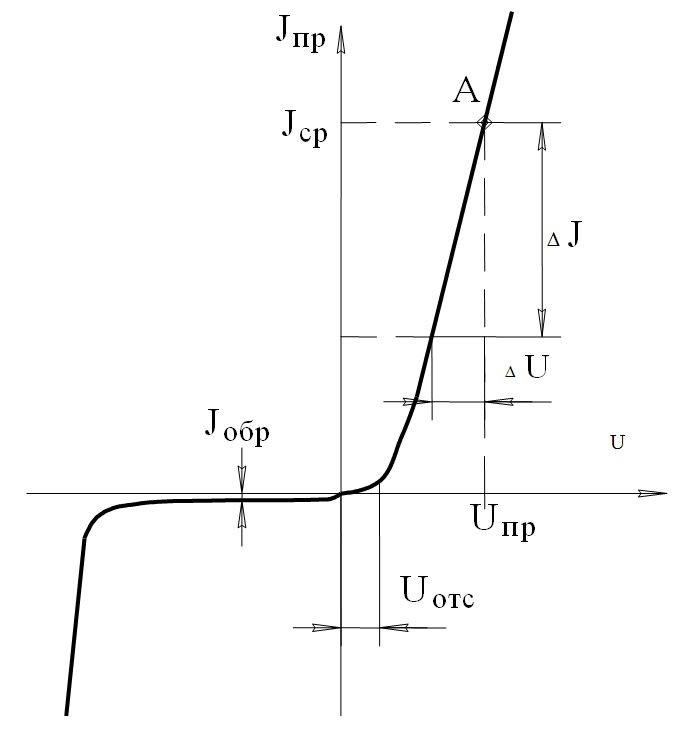
\includegraphics[width=0.4\textwidth]{2_VAC_of_diod.png}
\caption{ВАХ выпрямительного диода}
\label{fig:2_VAC_of_diod}
\end{figure}

Диоды обладают односторонней проводимостью и служат: для выпрямления переменного тока, стабилизации тока и напряжения, формирования импульсов, для регулирования мощностей и т.д.

Выпрямительные диоды применяются для преобразования переменного тока в постоянный. Они делятся: на маломощные (до 0,3А), средней мощности (до 10А), мощные (более 1000А), низкочастотные (до 1кГц) и высокочастотные (до 100кГц).

Свойства выпрямительных диодов характеризуются ВАХ и параметрами, которые приводятся в справочной литературе. Основные параметры диодов: средний выпрямленный ток Jср, прямое падение напряжения Uпр, обратный ток диода при заданной температуре Jобр., напряжение отсечки Uотс., мощность рассеивания Ррас., рабочая частота fр. и др.

Стабилитроны --- это разновидность диодов, предназначенных для стабилизации напряжения. Вольт – амперная характеристика стабилитрона имеет вид. Рабочий участок характеристики АВ лежит в области электрического пробоя диода и характеризуется малым изменением напряжения Uст при значительных изменениях тока.

Стабисторы, как и стабилитроны, предназначены для стабилизации напряжения. Однако, в отличие от последних, рабочим участком у них является прямая ветвь вольт–амперной характеристики. Стабисторы работают при прямом напряжении и позволяют стабилизировать малые напряжения (0,35 -- 1,9 В).

Варикапы – это полупроводниковые диоды, емкость которых меняется при изменении обратного напряжения.


% Вопрос 3 ------------------------------------------------------------
\quest{Полупроводниковые транзисторы. Классификация. Область применения.}

Транзистор — радиоэлектронный компонент из полупроводникового материала, обычно с тремя выводами, позволяющий входным сигналом управлять током в электрической цепи. Обычно используется для усиления, генерации и преобразования электрических сигналов. В общем случае транзистором называют любое устройство, которое имитирует главное свойство транзистора - изменения сигнала между двумя различными состояниями при изменении сигнала на управляющем электроде. Далее на схеме приведена классификация.

\begin{figure}[H]
\centering
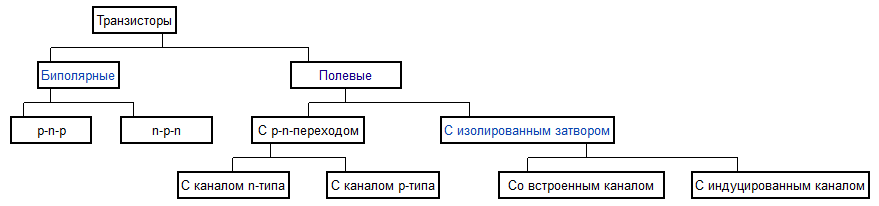
\includegraphics[width=1.0\textwidth]{3_Scheme_of_types.png}
\caption{Классификация транзисторов}
\label{fig:3_Scheme_of_types}
\end{figure}

Принцип действия биполярного транзистора основан на использовании физических процессов, происходящих при переносе основных носителей электрических зарядов из эмиттерной области в коллекторную через базу.

$I_\text{э} = I_\text{к} + I_\text{б}$, где $I_\text{э}$, $I_\text{к}$, $I_\text{б}$, – токи соответственно в цепи эмиттера, коллектора, базы.

Полевым транзистором называется транзистор, в котором между двумя электродами образуется проводящий канал, по которому протекает ток. Управление этим током осуществляется электрическим полем, создаваемым третьим электродом. Электрод, с которого начинается движение носителей заряда, называется истоком, а электрод, к которому они движутся, стоком. Электрод, создающий управляющее электрическое поле, называется затвором.


% Вопрос 4 ------------------------------------------------------------
\quest{Полупроводниковые резисторы. Классификация. Область применения.}

Полупроводниковые резисторы нашли широкое применение в электронных приборах. К ним относятся терморезисторы, магниторезисторы, варисторы, фоторезисторы. Принцип действия таких приборов основан на изменении свойств полупроводниковых материалов при воздействии на них температуры, магнитного и электрического полей, электромагнитного излучения.

Полупроводниковый терморезистор представляет собой прибор, сопротивление которого изменяется при изменении температуры. Зависимость сопротивления от температуры имеет вид:

\begin{equation}
R_{T}=A\exp{\frac{B}{T}}\text{, где}
\end{equation}
\par А, В --- постоянные, определяемые свойствами полупроводникового материала и конструкцией терморезистора;
\par Т --- температура.

С увеличением температуры сопротивление терморезистора уменьшается. Температурный коэффициент сопротивления терморезистора лежит в пределах от 2 до 8,5\% на градус.

Недостатком полупроводниковых терморезисторов является нелинейная зависимость сопротивления от температуры и значительный разброс параметров.

Терморезисторы применяются в качестве первичных преобразователей температуры для контроля и регулирования температуры, а также в схемах температурной компенсации.

Магниторезистор представляет собой полупроводниковый прибор, электрическое сопротивление которого зависит от воздействия на него магнитного поля. Магниторезисторы позволяют обеспечить хорошую гальваническую развязку. Для формирования магнитного поля можно использовать постоянный магнит или электромагнит.

Зависимость сопротивления магниторезистора от величины магнитного поля нелинейна. С увеличением величины магнитного поля сопротивление возрастает.

Основными параметрами магниторезистора являются:
\begin{itemize}
\item ном. сопротивление при отсутствии магнитного поля;
\item мощность рассеивания;
\item ТКR (температурный коэффициент сопротивления);
\item зависимость $R_{B} = f(H)$.
\end{itemize}


\begin{figure}[H]
\centering
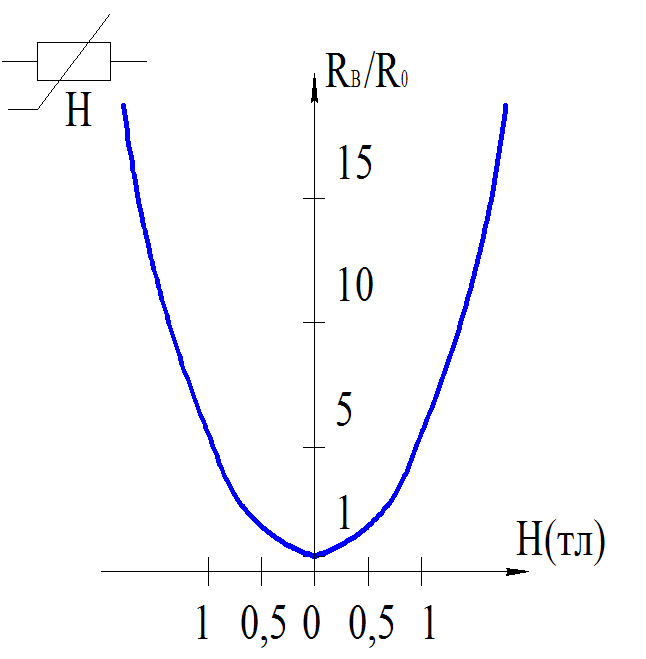
\includegraphics[width=0.35\textwidth]{4_R(H).png}
\hspace{1cm}
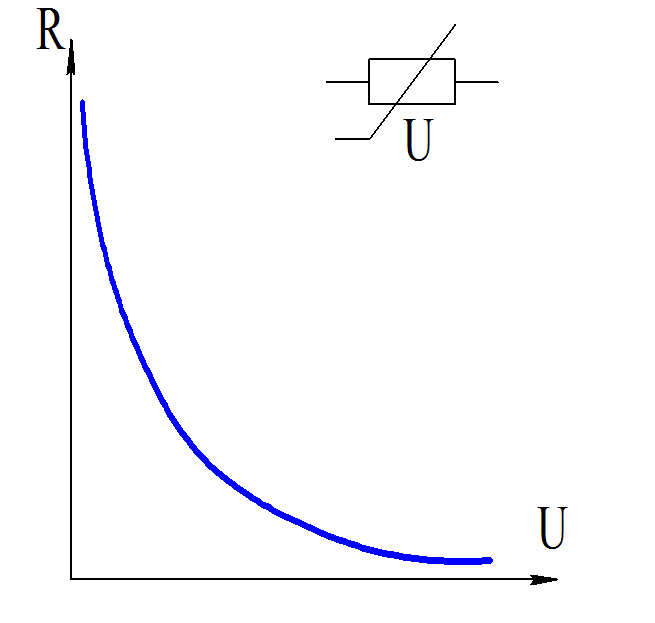
\includegraphics[width=0.35\textwidth]{4_R(U).png}
\\а) \hspace{0.4\textwidth} б)
\caption{Зависимости: R от H (а); R от U (б)}
\label{fig:4_R(U/H)}
\end{figure}

При увеличении магнитной индукции от 0 до 1 Тл сопротивление магниторезистора увеличивается в 10 - 15 раз. Магниторезисторы нашли применение в коммутационной технике: бесконтактных выключателях, реле, контактах управления. В настоящее время в приборостроении нашли широкое применение магнитодиоды, магнитотранзисторы, магнитотиристоры, которые представляют собой полупроводниковые приборы с p-n-переходами, параметры которых чувствительны к магнитному полю.

Варисторы представляют собой полупроводниковые резисторы, сопротивление которых зависит от приложенного напряжения. Зависимость сопротивления от напряжения нелинейная. Сопротивление RВ уменьшается при увеличении приложенного напряжения. Варисторы применяются для защиты от перенапряжений, защиты от помех, для искрогашения в электрических машинах. Они ограничивают возникающее напряжение, особенно при коммутации индуктивной или емкостной нагрузки и тем самым позволяют значительно повысить срок службы контактов реле и т.д.

Фоторезисторы представляют собой полупроводниковые приборы, сопротивление которых зависит от электромагнит. излучения.


% Вопрос 5 ----------------------------------------------------------
\quest{Фотоэлектрические приборы. Классификация. Область применения.}

Фотоэлектрические приборы строятся на принципах фотопроводимости.

Фотопроводимость – это свойство веществ изменять свою электропроводность под воздействием электромагнитного излучения.

Фотоэлектрические приборы делятся на две группы:
\begin{enumerate}
\item с внешним фотоэффектом
	\begin{itemize}
	\item вакуумные
	\item газонаполненные фотоэлементы (ФЭ)
	\item фотоэлектронные умножители (ФЭУ)
	\end{itemize}
\item с внутренним фотоэффектом
	\begin{itemize}
	\item фоторезисторы
	\item фотодиоды
	\item фототранзисторы
	\item фототиристоры
	\end{itemize}
\end{enumerate}

В качестве излучателей используется солнечный свет, лампочки накаливания и другие источники света.

Фотоэлемент (ФЭ) – это электровакуумный или газоразрядный диод, в стеклянном баллоне которого установлены фотокатод и фотоанод. Фотокатод представляет собой слой, покрывающий внутреннюю поверхность колбы, выполненный из полупроводникового материала, чувствительного к внешнему излучению. Анод выполнен в виде кольца или рамки и размещен внутри колбы. ФЭ разделяются на вакуумные и газоразрядные.

При отсутствии излучения анодный ток равен нулю. При освещении фотокатода возникает фотоэмиссия, и в цепи анода протекает ток.

Фотоэлементы используются в первичных преобразователях информации.

Фотоэлектронный умножитель представляет собой электровакуумный прибор, преобразующий энергию электромагнитного излучения в электрические сигналы с использованием вторичной электронной эмиссии. Состоит из стеклянного баллона, внутри которого расположены ускоряющие электроды, умножительные электроды и анод. При освещении фотокатода возникает электронный поток, который фокусируется и направляется на умножительные электроды, где за счет вторичной эмиссии он усиливается и попадает на анод.

Фоторезистор представляет собой полупроводниковый прибор, сопротивление которого зависит от освещенности.

Фотодиод представляет собой полупроводниковый прибор с n-p переходом. Принцип работы фотодиода заключается в том, что при его освещении возрастает обратный ток, и он не зависит от обратного напряжения. На границе перехода “n-p” возникает ЭДС, величина которой зависит от освещенности и может достигать 0,5 - 1 В. При этом обратное сопротивление фотодиода уменьшается.

Они относятся к быстродействующим приборам и реагируют на сигналы до 1 МГц. Фотодиоды могут также использоваться в качестве источников питания, например, в солнечных батареях.

Фототранзистор в отличие от фотодиода является активным преобразователем, в нем происходит не только преобразование энергии излучения, но и усиление.
Внутренний фотоэффект в полупроводнике может быть использован для построения других приборов, например, фототиристоров, однопереходных фототранзисторов и др.


% Вопрос 6 ----------------------------------------------------------------------
\quest{Аналоговые усилители. Классификация. Основные характеристики и параметры.}

Усилитель - устройство, предназначенное для усиления электрических сигналов по напряжению, току или мощности за счет преобразования энергии источника питания в энергию выходного сигнала. Усилитель включает в себя нелинейный элемент, управляемый входным электрическим сигналом $U_\text{вх}$, источник питания $U_\text{п}$ и нагрузочное устройство с сопротивлением $Z_\text{н}$. Аналоговые усилители служат для усиления аналоговых сигналов.

Классификация усилителей производится по многим признакам:
\begin{itemize}
\item по виду усиливаемого:
	\begin{itemize}
	\item гармонических сигналов
	\item импульсных сигналов
	\end{itemize}
\item по типу усиливаемого сигнала:
	\begin{itemize}
	\item напряжения
	\item тока 
	\item мощности
	\end{itemize}
\item по диапазону усиливаемых частот:
	\begin{itemize}
	\item постоянного тока 
	\item переменного тока. Которые в зависимости от диапазона усиливаемых частот делятся на:
		\begin{itemize}
		\item усилители низкой частоты (УНЧ)
		\item высокой частоты (УВЧ)
		\item широкополосные
		\item избирательные усилители.
		\end{itemize}
	\end{itemize}
\item по виду нагрузки:
	\begin{itemize}
	\item с активной нагрузкой
	\item c активно-индуктивной нагрузкой
	\item c емкостной нагрузкой
	\end{itemize}
\item по количеству каскадов:
	\begin{itemize}
	\item однокаскадные 
	\item многокаскадные. Связь в между каскадами может быть:
		\begin{itemize}
		\item гальванической
		\item емкостной
		\item индуктивной
		\end{itemize}
	\end{itemize}
\end{itemize}

Основными характеристиками любого усилителя являются:
\begin{itemize}
\item амплитудная характеристика, которая представляет собой зависимость $U_\text{выx} = \varphi(U_\text{вх})$. Для линейных усилителей это прямая, проходящая через начало координат;
\item амплитудно-частотная характеристика (АЧХ) $U_\text{выx} = \varphi(f)$ отражает зависимость амплитуды выходного сигнала от частоты. Реально в усилителях из-за наличия паразитных емкостей и индуктивностей различные частоты усиливаются неодинаково;
\item фазо-частотная характеристика $U_\text{выx} = \lambda(f)$ отражает зависимость угла сдвига фазы выходного сигнала по отношению к фазе входного сигнала;
\item переходная характеристика – отражает реакцию усилителя на единичный скачок входного напряжения. Переходная характеристика определяется по ее изображению на экране осциллографа при подаче на вход усилителя входного сигнала прямоугольной формы. Процесс изменения выходного сигнала может быть колебательным либо апериодичным.
\end{itemize}

Важнейшими параметрами усилителя являются:
\begin{itemize}
\item коэффициент усиления по току $K_{I} = \dfrac{\Delta I_\text{вых}}{\Delta I_\text{вх}}$
\item коэффициент усиления по напряжению $K_{U} = \dfrac{\Delta U_\text{вых}}{\Delta U_\text{вх}}$
\item коэффициент усиления по мощности $K_{P} = \dfrac{\Delta P_\text{вых}}{\Delta P_\text{вх}}$
\end{itemize}

Полоса пропускания усилителя $2\Delta f$ характеризует частотные свойства усилителя. Измеряется на уровне $0,707 K_{max}$

Для наглядности в ряде случаев АЧХ строится в относительных единицах усиления.
\begin{equation}
N(F) = \dfrac{K(f)}{K_{max}}\text{, где}
\end{equation}
\par $K(f)$ --- коэффициент усиления на частоте $f$;
\par $K_{max}$ --- максимальный коэффициент усиления.

Входное и выходное сопротивление необходимо учитывать при согласовании с источником входного сигнала и с нагрузкой. 

Выходная мощность усилителя – это мощность, которая выделяется на нагрузке.

Искажения сигналов в усилителе – это отклонение формы выходного сигнала от формы входного сигнала. Различают два вида искажений: статические (нелинейные) и динамические (линейные). Нелинейные искажения возникают в усилителе за счет работы его на нелинейном участке ВАХ. Количественно нелинейные искажения оцениваются коэффициентом нелинейных искажений.
\begin{equation}
K_{H} = \dfrac{\sqrt{(A_{2}^{2} + A_{3}^{2} + \ldots + A_{n}^{2})} }{A_{1}}\text{, где}
\end{equation}
\par $A_{n}$ --- амплитуда n-й гармоники;
\par $A_{1}$ --- амплитуда основной гармоники выходного сигнала.

Линейные искажения определяются амплитудно-частотной характеристикой усилителя и количественно оцениваются коэффициентами частотных искажений на низких и высоких частотах.

Для получения высоких коэффициентов усиления в состав усилителя входит обычно несколько каскадов. Первым каскадом, как правило, является предварительный усилитель, затем идут промежуточный усилитель и усилитель мощности. Предварительный усилитель обеспечивает связь источника сигнала с усилителем. Он должен иметь большое входное сопротивление для того, чтобы не ослаблять входной сигнал. Промежуточный усилитель обеспечивает основное усиление, а усилитель мощности обеспечивает заданную выходную мощность.

При построении усилительных устройств наибольшее распространение получили каскады на биполярных и полевых транзисторах, включенных с ОЭ (OU) или с ОК (OC).


\quest{Избирательные усилители. Усилители постоянного тока. Усилители мощности. Область применения.}
\quest{Операционные усилители. Классификация. Область применения. Балансировка ОУ.}

Операционным усилителем называют усилитель постоянного тока, предназначенный для выполнения различного рода операций над аналоговыми сигнала при работе в схемах с отрицательной обратной связью.

Операционные усилители обладают большим и стабильным коэффициентом усиления напряжения, имеют дифференциальный вход с высоким входным сопротивлением и несимметричный выход с низким выходным сопротивлением, малым дрейфом нуля. То есть под операционным усилителем понимают высококачественный универсальный усилитель.

Условные обозначения операционных усилителей приведены на рис. 3.50. Один из входов, обозначенный знаком «+» называют неинвертирующим (прямым), так как сигнал на выходе и сигнал на этом входе имеют одинаковую полярность. Второй вход, обозначенный знаком «–», (его также обозначают знаком инверсии «o») называют инвертирующим, так как сигнал на выходе по отношению к сигналу на этом входе имеет противоположную полярность. Помимо трех сигнальных контактов (двух входных и одного выходного) операционный усилитель содержит дополнительные контакты (обычно число контактов составляет 14 или 16).
\begin{figure}[H]
\centering
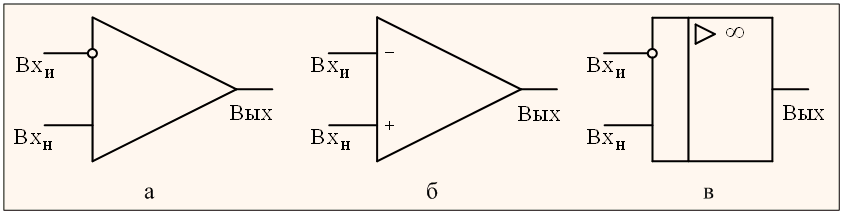
\includegraphics[width=0.7\textwidth]{8_oa_graphic.png}
\caption{УГО операционного усилителя}
\label{fig:8_oa_graphic}
\end{figure}

Параметры операционного усилителя характеризуют его эксплуатационные возможности. Основными параметрами являются:
\begin{enumerate}
\item Коэффициент усиления напряжения без обратной связи $K_{u}$, показывающий, во сколько раз напряжение на выходе превышает напряжение сигнала, поданного на дифференциальный вход. Типовое значение $K_{u} = 10^{5} \div 10^{6}$;
\item Коэффициент ослабления синфазного сигнала $K_\text{осл.сф}$, показывающий, во сколько раз дифференциальный сигнал сильнее синфазного. Донный параметр определяется свойствами входного дифференциального каскада и составляет $80 \div 100$ дБ;
\item Напряжение смещения нуля $U_\text{см}$, представляющее собой постоянное напряжение определенной полярности, которое необходимо подать на вход при отсутствии входного сигнала для того, чтобы напряжение на выходе стало равным нулю. Наличие отклонения выходного напряжения от нуля обусловлено, хотя и малым, но неизбежным дисбалансом плеч дифференциального каскада. Практически $U_\text{см} = 5 \div 20$ мВ;
\item Температурный дрейф напряжения смещения $TKU_\text{см} = \dfrac{\Delta U_\text{см}}{\Delta T}$, характеризует изменение напряжения $U_\text{см}$ при изменении температуры и составляет $1 \div 30 \dfrac{\text{мкВ}}{\text{\textcelsius}}$;
\item Входное сопротивление для дифференциального сигнала $R_\text{вх. диф}$. Измеряется со стороны любого входа в то время, когда другой вход соединен с общим выводом. Величина $R_\text{вх. диф}$ лежит в пределах сотен кОм – единиц МОм;
\item Входное сопротивление для синфазного сигнала $R_\text{вх. сф}$. Измеряется между соединенными вместе входами операционного усилителя и корпусом. Данное сопротивление на несколько порядков больше чем сопротивление для дифференциального сигнала;
\item Выходное сопротивление $R_\text{вых}$. Величина выходного сопротивления для операционного усилителя составляет десятки – сотни Ом.
\end{enumerate}

В соответствии со значениями основных параметров многообразие выпускаемых ОУ можно разделить на несколько разновидностей:

\begin{enumerate}
\item Универсальные усилители общего назначения составляют большую часть номенклатуры ОУ. Это дешевые усилители среднего быстродействия, невысокой точности и малой выходной мощности, с  типичными параметрами: Ku = $10^{3} - 10^{5}$, f1 = 0.1 - 10 МГц и напряжение смещения нулевого уровня Uсм = 0.1 - 10 мВ.

\item Прецизионные усилители характеризуются суммарной погрешностью не более долей процента и при среднем быстродействии имеют высокий коэффициент усиления напряжения, малое напряжение смещения нуля, большой коэффициент подавления синфазного сигнала, малый входной ток и низкий уровень шума.

\item Быстродействующие усилители имеют высокую частоту единичного усиления f1 = 50 - 1000 МГц и обеспечивают скорость нарастания выходного сигнала Vu= 10 - 1000 В/мкс при средних точностных параметрах.

\item Микромощные усилители потребляют очень малый ток Iпит порядка 1 мкА при небольших уровнях напряжения электропитания Uпит = $\pm 0.9 - \pm 5$ В. Все другие параметры (особенно быстродействие) у них обычно невысокие. Эти усилители используют в приборах с автономным электропитанием от гальванических или аккумуляторных батарей.

\item Мощные и высоковольтные усилители имеют разность положительного и отрицательного питающих напряжений свыше 50 В и выходной ток 0.1 - 1А, а некоторые модификации допускают токи до 10 - 100 А и мощности свыше 100 Вт.
\end{enumerate}

ОУ имеет два вывода балансировки (на рисунке обозначены Offset), которые обеспечивают возможность подстройки напряжения смещения входа ОУ до нулевого значения. Для подстройки нужно подключить к выводам потенциометр.


% Вопрос 9 --------------------------------------------------------------------
\quest{Стабилизаторы напряжения. Классификация. Параметры. Область применения.}

Стабилизатор напряжения — преобразователь электрической энергии, позволяющий получить на выходе напряжение, находящееся в заданных пределах при значительно больших колебаниях входного напряжения и сопротивления нагрузки.

По типу выходного напряжения стабилизаторы делятся на стабилизаторы постоянного тока и переменного тока. Как правило, тип питания (постоянный либо переменный ток) такой же, как и выходное напряжение, хотя возможны исключения.

Стабилизаторы напряжения подразделяются на однофазные и трехфазные стабилизаторы напряжения.

По типам конструкции стабилизаторы напряжения делятся на:
\begin{itemize}
\item феррорезонансные. Принцип действия основывается на магнитном насыщении сердечников из ферромагнетиков трансформаторов. Этот тип стабилизаторов напряжения был разработан достаточно давно, в начале 60-х годов прошлого века и был призван защитить сложную бытовую технику. Но в настоящее время от их производства отказались почти все производители, из-за очень узкого рабочего диапазона напряжений и невозможности работы прибора без нагрузки.
\item электромеханические. В стабилизаторах этого типа корректировка напряжения производится автоматически, а точность поддержания напряжения достаточно высока (в пределах 3\%).
\item электронные. Этот тип стабилизаторов работает по принципу автоматического переключения трансформаторных секций при помощи силовых ключей (реле, тиристоров и т.д.). Электронные стабилизаторы ступенчатого регулирования обеспечивают выходное напряжение в более широких пределах, чем электромеханические. А также обладают высоким быстродействием и не изменяют форму входного напряжения.
\end{itemize}

Основными параметрами стабилизатора напряжения являются:
\begin{itemize}
\item Диапазон входных напряжений(Диапазон напряжений в пределах которого стабилизатор может поддерживать выходное напряжение с заданной точностью)
\item Диапазон  выходных напряжений (Диапазон возможных значений)
\item Точность поддержания выходного напряжения в \%
\item Мощность стабилизатора. Обычно указывается в кВа, это полная мощность.
\end{itemize}

Выбор стабилизатора:
\begin{enumerate}
\item Для выбора стабилизатора необходимо посчитать сумму полных мощностей потребителей, если на потребителе указан $\cos\varphi$ (коэфф. активном мощности в полной), то его учитываем.
\item Определить диапазон изменений напряжений в сети. Произвести изменения максимальных и минимальных напряжений.
\item Выяснить диапазон рабочих напряжений потребителей
\end{enumerate}


% Вопрос 10 ------------------------------------
\quest{Логические операции. Схемная реализация.}

Логическая операция — операция над выражениями булевского типа, соответствующая некоторой операции над высказываниями в алгебре логики. Как и высказывания, логические выражения могут принимать одно из двух истинностных значений — «истинно» или «ложно». Логические операции служат для получения сложных логических выражений из более простых. В свою очередь, логические выражения обычно используются как условия для управления последовательностью выполнения программы.
Обычно выделяют следующие базовые операции:
\begin{itemize}
\item НЕ (отрицание)
\item И (конъюнкция)
\item ИЛИ (дизъюнкция)
\item XOR (исключающее ИЛИ)
\end{itemize}
Для каждой из операции можно построить простую таблицу истинности.

\begin{figure}[H]
\centering
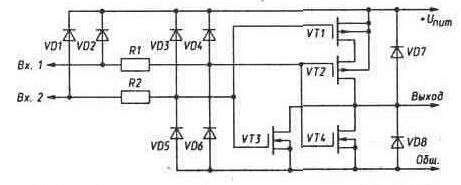
\includegraphics[width=0.7\textwidth]{10_or_not.png}
\caption{Схемная реализация ИЛИ-НЕ}
\label{fig:10_or_not}
\end{figure}
Для всех микросхем существует УГО.


% Вопрос 11 ---------------------------------------------------------------------------------------------------------------
\quest{Цифровые устройства. Классификация. Комбинационные ЦУ. Дешифраторы, шифраторы, мультиплексоры, демультиплексоры.}
% Вопрос 12 ---------------------------------------------------------------------------------------------------------------
\quest{Комбинационные сумматоры.}
% Вопрос 13 ---------------------------------------------------------------------------------------------------------------
\quest{Триггера. Классификация. Область применения.}
% Вопрос 14 ---------------------------------------------------------------------------------------------------------------
\quest{Регистры и счетчики. Классификация. Схемы. Область применения.}
% Вопрос 15 ---------------------------------------------------------------------------------------------------------------
\quest{Цифро-аналоговые преобразователи. Назначение. Принцип работы. Матрица R-2R. Область применения.}
% Вопрос 16 ---------------------------------------------------------------------------------------------------------------
\quest{Аналого-цифровые преобразователи. Классификация. Область применения. Параллельные АЦП. АЦП поразрядного взвешивания.}
% Вопрос 17 ---------------------------------------------------------------------------------------------------------------
\quest{Интегрирующие АЦП. АЦП двойного интегрирования.}
% Вопрос 18 ---------------------------------------------------------------------------------------------------------------
\quest{Таймеры. Классификация. Область применения.}
% Вопрос 19 ---------------------------------------------------------------------------------------------------------------
\quest{Источники вторичного напряжения. Структурные схемы. Выпрямители и фильтры.}
% Вопрос 20 ---------------------------------------------------------------------------------------------------------------
\quest{Транзисторный усилительный каскад с общим эмиттером.}
% Вопрос 21 ---------------------------------------------------------------------------------------------------------------
\quest{Дискретные цифровые САР: математическое описание, Z передаточные функции.}
% Вопрос 22 ---------------------------------------------------------------------------------------------------------------
\quest{Анализ дискретных САР.}
% Вопрос 23 ---------------------------------------------------------------------------------------------------------------
\quest{Логарифмические частотные характеристики САР.}
% Вопрос 24 ---------------------------------------------------------------------------------------------------------------
\quest{Переходные функции и переходные характеристики САР. Реакция САР на произвольный входной сигнал.}
% Вопрос 25 ---------------------------------------------------------------------------------------------------------------
\quest{Типовые звенья САР и их частотные и временные характеристики.}
% Вопрос 26 ---------------------------------------------------------------------------------------------------------------
\quest{Устойчивость линейных САР: определение, теоремы Ляпунова, алгебраический критерий устойчивости Гурвица.}
% Вопрос 27 ---------------------------------------------------------------------------------------------------------------
\quest{Частотные критерии устойчивости линейных САР.}
% Вопрос 28 ---------------------------------------------------------------------------------------------------------------
\quest{Анализ качества линейных САР.}
% Вопрос 29 ---------------------------------------------------------------------------------------------------------------
\quest{Синтез корректирующих устройств линейных САР.}
% Вопрос 30 ---------------------------------------------------------------------------------------------------------------
\quest{Анализ нелинейных САР.}
% Вопрос 31 ---------------------------------------------------------------------------------------------------------------
\quest{Показатели качества ЭС.}

Показатели качества продукции – количественная характеристика определенного свойства продукции на определенном этапе жизненного цикла.

Показатели качества продукции делятся на следующие группы:
\begin{enumerate}
\item Назначения
\item Надежности
\item Технологичности
\item Эргономические
\item Эстетические
\item Стандартизация и унификация
\item Патентно-правовые
\item Экономические
\end{enumerate}

Единичный показатель качества --- показатель качества продукции, относящийся только к одному из её свойств. Комплексный показатель качества --- показатель качества продукции, относящийся к нескольким её свойствам.

% Вопрос 32 ---------------------------------------------------------------------------------------------------------------
\quest{Управление качеством ЭС.}

Управление качеством продукции базируется на статических методах контроля, зародилось в 30-е годы в связи с переходом к массовому производству изделий. В связи с этим стали применять выборочный контроль продукции с оценкой его результатов статистическим методом.
Контроль качества базируется на статистических методах и развиваясь циклически проходит через определенные этапы (см. рис)
\begin{center} 
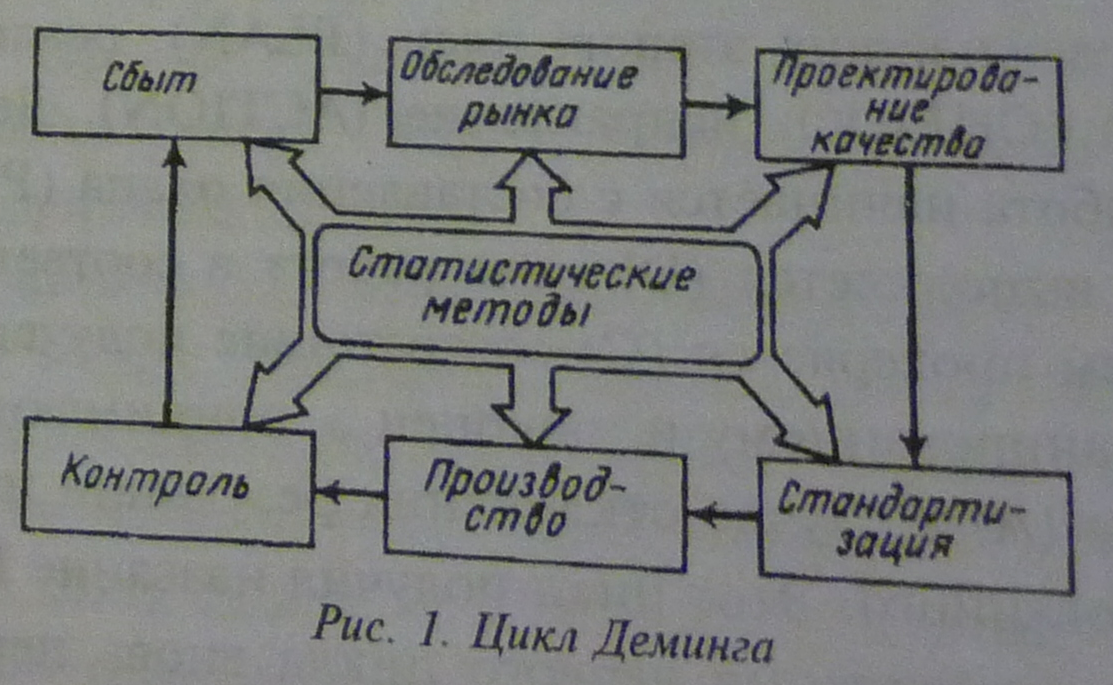
\includegraphics[width=0.6\textwidth]{32_Demming.png}\\
\end{center}

Управление качеством продукции базируется на статических методах контроля, зародилось в 30-е годы в связи с переходом к массовому производству изделий. В связи с этим стали применять выборочный контроль продукции с оценкой его результатов статистическим методом.

Контроль качества базируется на статистических методах и развиваясь циклически проходит через определенные этапы

Для эффективного обеспечения контроля качества необходимо участие всех, без исключения, работников предприятия. Такой контроль качества называется Тотальным(TQC). Был придуман и внедрен впервые в Японии 60х годах.

Среди статистических методов можно выделить 7 наиболее эффективных и доступных:
\begin{enumerate}
\item	Расслоение графики (полигон, гистограмма, кумулятивная кривая)
\item	Расслоение общей изменчивости статистических данных с помощью дисперсионного анализа.
\item	Диаграмма Парето
\item	Причинно-следственная диаграмма
\item	Диаграмма разброса (поле корреляции)
\item	Контрольная карта
\item	Контрольный лист
\end{enumerate}


% Вопрос 33 ---------------------------------------------------------------------------------------------------------------
\quest{Себестоимость и уровень качества ЭС.}

Зависимость себестоимости и уровня качества продукции можно в общем виде представить в виде следующего графика (рис.3)

СП – затраты на материалы, комплектующие  изделия, оборудование, заработную плату, контроль и испытания и т.д. 
 \begin{center} 
 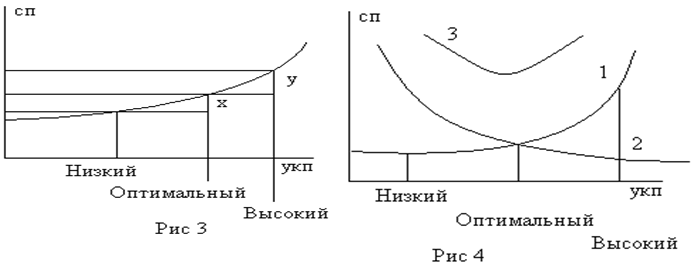
\includegraphics[width=0.7\textwidth]{33_Sebestoim.png}
 \end{center}
При повышении уровня качества от низкого до оптимального затраты растут медленно (х), поскольку производство легко справляется с заданными требованиями на уровень качества. По мере повышения УКП затраты (у) существенно возрастают. При дальнейшем повышении требований к УКП в конце концов достигается такой предел, когда ни оборудование, ни ТП, ни НТП и т.д. не в состоянии обеспечить требуемого (недостижимо высокого) качества. Затраты при этом устремляются в бесконечность.

Затраты на продукцию складываются из затрат на изготовление (проектирование и производство) и на эксплуатацию продукции (рис. 4).
Оптимальный уровень качества продукции - это такой уровень, выше или ниже которого производить продукцию экономически нецелесообразно.
При низком уровне качества продукции в сфере эксплуатации потребитель вынужден выделять дополнительные средства на ремонт, доработку и обслуживание продукции.
Высокий уровень качества продукции обуславливается ее высокой себестоимостью. 


\begin{enumerate}
\item Расслоение графики (полигон, гистограмма, кумулятивная кривая)
\item Расслоение общей изменчивости статистических данных с помощью дисперсионного анализа.
\item Диаграмма Парето
\item Причинно-следственная диаграмма
\item Диаграмма разброса (поле корреляции)
\item Контрольная карта
\item Контрольный лист
\end{enumerate}


% Вопрос 34 ---------------------------------------------------------------------------------------------------------------
\quest{Корреляционная связь показателей ЭС.}

Диаграмма разброса применяется для исследования зависимости (корреляции) между двумя видами данных. Поэтому её часто называют полем корреляции.
С помощью диаграммы разброса удобно наблюдать процесс изменения параметра качества во времени при воздействии тех или иных факторов.

Совокупность точек на графике – диаграмма рассеяния.
С помощью диаграммы разброса можно определить имеется ли связь между параметрами и вид корреляции.(прямая корреляция, легкая прямая корреляция, обратная корреляция, легкая обратная корреляция, отсутствие корреляции, криволинейная корреляция.)

 \begin{center} 
 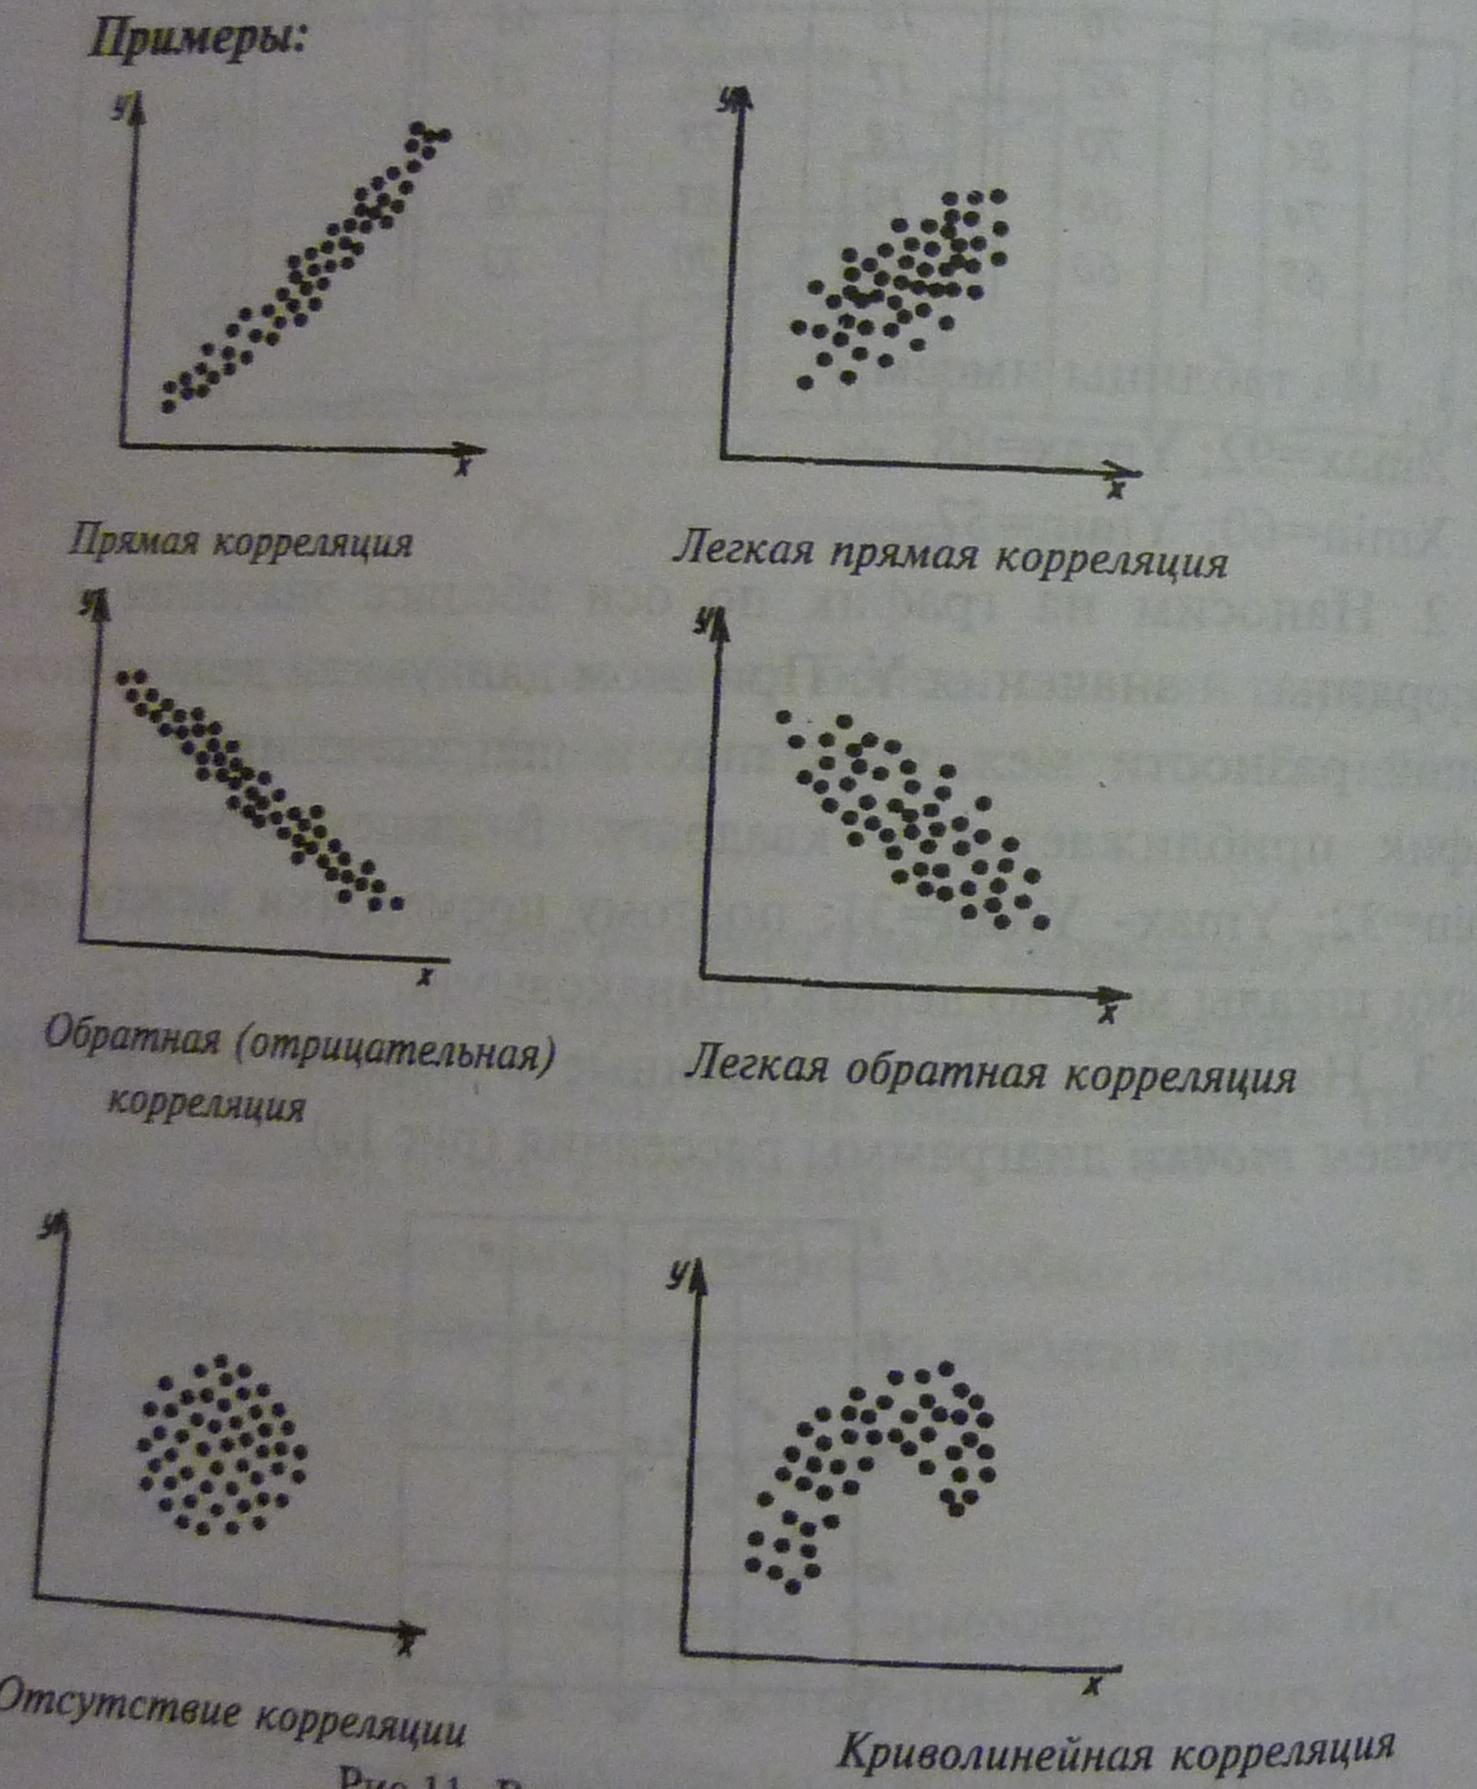
\includegraphics[width=0.5\textwidth]{34_Korelyacia.png}
 \end{center}
 
 Криволинейную корреляцию можно разделить на участки, имеющие прямолинейный характер, и исследовать каждый участок в отдельности.
 
 Степень связи может быть оценена: коэффициентом корреляции (прямолинейная), корреляционным отношением (криволинейная).
 
 Связь прямолинейную между Х и У можно найти:
 \begin{equation}
 Y-m_Y = r \cdot \frac{S_X}{S_Y} \cdot (X-m_Y),
 \end{equation}
 где r - коэффициент парной корреляции,
 \begin{equation}
 r = \frac{\sum_{i=1}^n (X_i - m_X)(Y_i-m_Y)}{(n-1) \cdot S_X \cdot S_Y},
 \end{equation} 
 \begin{equation}
 m_X = \dfrac{\sum_{i=1}^n X_i}{n}; S_X=\sqrt{\dfrac{\sum_{i=1}^n (X_i -m_X)^2}{n-1}},
 \end{equation}
 
  n - число пар наблюдений.
  
 $ -1 \leqslant r \leqslant 1$
 
 При |r|=1 – связь функциональная (зависимость между параметрами ввиде формул),
 
при |r|<1 – связь статическая. Каждому фиксированному значению Х соответствует ряд изменяющихся вместе с Х значений У и наоборот. Параметры Х и У считаются статистически зависимыми, если
\begin{center} 
  $\dfrac{\mid r \mid \cdot \sqrt{n-2}}{\sqrt{1-r^{2}}} \geqslant t_T = f(\alpha ; \nu = n-2)$\\
  \end{center}
  
Знак говорит о связи значений, если «-» то при уменьшении значения Х , У увеличивается и наоборот. Если «+» то при увеличении Х увеличивается и У.
  При r = 0 Х и У не связаны  между собой и не зависят друг от друга.

% Вопрос 35 ---------------------------------------------------------------------------------------------------------------
\quest{Метод расслаивания <<4М>>.}

Простой и эффективный статистический метод, широко используемый в системе УК, - метод расслаивания

В основе метода – расслаивание статистических данных (т.е. группировка данных) в зависимости от условия их получения и обработка каждой группы в отдельности. Данные, разделённые на группы в соответствии с их особенностями, называют слоями (стратами), а сам процесс разделения на слои – расслаиванием (стратификацией). Существуют различные методы расслаивания, применение которых зависит от конечных задач. В производственных условиях обычно используется метод 4М, учитывающий факторы, зависящие от человека, машины, материала, метода. Расслаивание осуществляется:
\begin{enumerate}
\item по исполнителям – квалификации, полу, стажу работы и т.п.;
\item по оборудованию – году выпуска, марке, типу конструкции  и т.п.;
\item по материалу – месту производства, фирме-производителю и т.п.;
\item по способу производства 

\end{enumerate}

В результате расслаивания обязательно должны соблюдаться два условия:
\begin{itemize}
\item различия между значениями СВ внутри слоя должны быть как можно меньше по сравнению с различием её значений в не расслоенной исходной совокупности;
\item различие между слоями  должно быть как можно больше.
\end{itemize}	

При контроле качества изготовления изделий на практике возникает задача предполагаемого источника ухудшения качества продукции, когда разброс значений параметра качества около среднего значения возрастает. В случае нормального закона распределения контролируемого параметра качества такую информацию возможно получить путём расслаивания дисперсии с помощью дисперсионного анализа.

% Вопрос 36 ---------------------------------------------------------------------------------------------------------------
\quest{Метод <<АВС-анализ>>.}

Метод служит для эффективности контроля качества изделия, для этого все изделия разбиваются по ценовым диапазонам (или иным критериям), составляется таблица,\\
\begin{center} 
  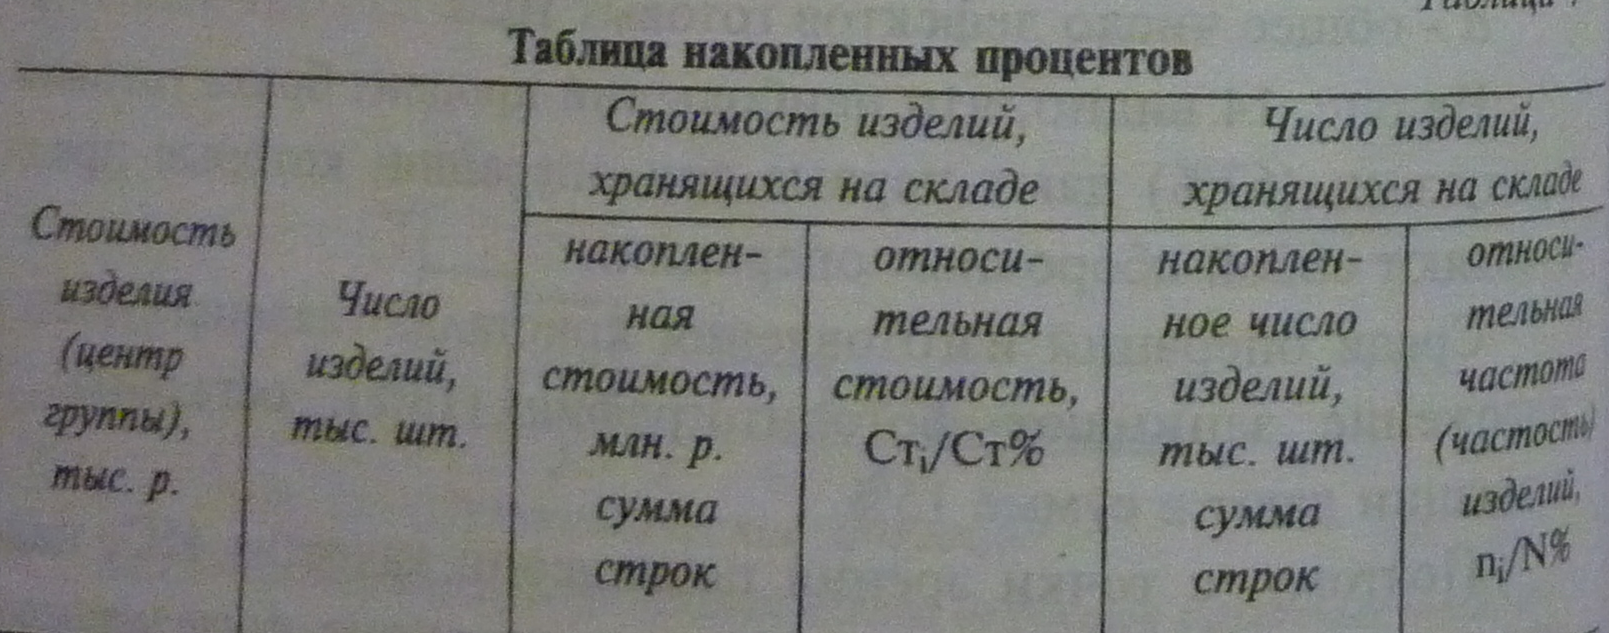
\includegraphics[width=0.7\textwidth]{36_Shapka.png}
  \end{center}
   и строится диаграмма Парето (по оси У откладывается относительная стоимость изделия в 
   \textdiscount
   , а по оси Х относительная частость изделий в
  \textdiscount). По результатам которой можно выделить три группы: группа А – наиболее дорогие изделия и её контроль должен быть наиболее строгим, группа С – наиболее дешевые изделия и её контроль упрощенный, все остальные изделия отнесутся к группе В и контроль качества должен быть средним.
  АВС-анализ широко применяется для контроля за производительностью труда, контроля денежных сумм, связанных со сбытом  и т.д.
  
\quest{Виды статистического контроля ЭС.}
%Вопрос №37

Статистический контроль – это процесс установления соответствия между состоянием объекта и заданными на него нормами.\\
Контролем охватываются все этапы производства ЭС. В зависимости от стадии жизни изделия различают производственный и эксплуатационный контроль.

\underline{Производственный контроль} – (статический на стадии производства) охватывает все вспомогательные, подготовительные и технологические операции. В зависимости от места в цепи ТП произв контроль подразделяют на входной, операционный и приемочный.\\
\textit{Входной контроль} – контроль продукции поставщика. Материалы, комплектующие изделия подвергаются контролю на соответствие НТД.\\
\textit{Операционный контроль} – контроль продукции после завершения определенной операции.\\
\textit{Приемочный контроль} – контроль готовой продукции по окончании всех технологических операций.

\underline{Эксплуатационный контроль} – контроль, осуществляемый на стадии эксплуатации.\\
Часто статический контроль называют параметрическим контролем, потому что он базируется на контроле фактических значений параметров качества и сравнении их с запланированными значениями по НТД.

Перечисленные виды контроля могут быть как сплошными (100\textdiscount), так и выборочными.\\
Контроль по количественному признаку – регистрация точных числовых значений, измеряемых параметров качества.

Контроль по качественному признаку – выделяются категории к которым принадлежит контролируемое изделие. Частным случаем контроля по качественному признаку является контроль по альтернативному признаку – когда продукция разбивается на годную и не годную.
Летучий контроль – выборка из потока изделий в случайное время для контроля.

\quest{Количественные показатели надежности ЭС.}
%Вопрос №38

Виды изделий:
	\begin{enumerate}
	\item По способу применения (изделия однократного и многократного действия);
\item	По способу обслуживания (восстанавливаемые и невосстанавливаемые изделия).
	\end{enumerate}
Восстанавливаемое ЭС -  изделие, изделия отказы которого устраняются путем ремонта (замены отказавшего элемента работоспособным). При этом само изделие состоит из невосстанавливаемых ЭРЭ (резисторов, конденсаторов, ИС) и узлов (собранных на гибридных и твердых схемах, микромодулях, микропроцессорах). Отказавшие ЭРЭ и узлы изымаются из изделия и заменяются на работоспособные.
Невосстанавливаемые являются изделия, не подлежащие ремонту в процессе эксплуатации.
\begin{itemize}
\item 	Показатели надежности  являются случайными величинами, т.к. все отказы случайные события
\item	Показатели надежности – функции времени.
	\end{itemize}
Показатели (их 5):
\begin{enumerate}


\item \underline{	Вероятность безотказной работы} p(t) – вероятность того что в заданном интервале времени (от 0 до t часов) в изделии не произойдет отказа.\\
p(t) = P(T>t), где Т – время безотказной работы, t – заданное время работы изделия.

Статистический расчет \\
\begin{equation}
p^{*}(t) = \frac{N(t)}{N_0} = \frac{N_0 - n(t)}{N_0} = 1- \frac{n(t)}{N_0}
\end{equation}, где $N_0$ – общее число изделий, n(t) – число изделий отказавших за время t, N(t) – число изделий продолжающих работать после времени t.\\
$0 \leqslant p^{*}(t) \leqslant 1$.

Вероятность безотказной работы может быть и определена и для произвольного интервала времени (t1,t2). В этом случае говорят об условной вероятности безотказной работы
$P(t1,t2) = \frac{ P(t2)}{P(t1)}$
\item  \underline{	Вероятность отказа}q(t) - вероятность того что изделие откажет в течении заданного интервала времени (от 0 до t часов).
$q(t) = P(T \leqslant 1)$,
\begin{equation}
q(t) = 1-p(t),
\end{equation}
 вероятность отказа – противоположное событию безотказной работы.
 
Статистически значение находится по формуле\\
\begin{equation} q^{*}(t) = 1-p^{*}(t) = 1-1+\frac{n(t)}{N_0}=\frac{n(t)}{N_0},
\end{equation}
$0 \leqslant q^{*}(t)\leqslant 1$
\item	\underline{Частота отказов} f(t) – представляет безусловную плотность вероятности безотказной работы изделия. Она производная по времени от функции вероятности отказа\\
\begin{equation}f(t) = \frac{dq(t)}{dt} = -\frac{dp(t)}{dt} ,
\end{equation}
Частота отказа характеризует скорость изменения надежности (по вероятности безотказной работы) во времени, причем изменение происходит в сторону снижения надежности.

Статистически  она находится по формуле
\begin{equation}f^{*}(t) = \frac{n(t+\Delta t)-n(t)}{\Delta t \cdot N}= \frac{n(t)}{\Delta t \cdot N},
\end{equation} где $n(t+ \Delta t)$ – число отказавших изделий за время $ t+\Delta t$ \\
$f^{*}(t)$ – отношение числа отказавших изделий  в единицу времени t к общему числу изделий поставленных на испытания $N_0$.

\item \underline{Интенсивность отказов} $\lambda (t)$ – условная плотность вероятности безотказной работы.
\begin{equation} \lambda (t) = -  \frac{dp(t)}{dt} \cdot \frac{1}{p(t)} =  \frac{f(t)}{p(t)},
\end{equation}

Статистически интенсивность находят как\\
\begin{equation} \lambda^{*}(t)=\frac {f^{*}(t)}{p^{*}(t)}=\frac{n(\Delta t)}{\Delta t \cdot N(t)}
\end{equation}

Графическая зависимость интенсивности отказов от времени для большинства ЭС имеет вид\\
\begin{figure}[H]
\centering
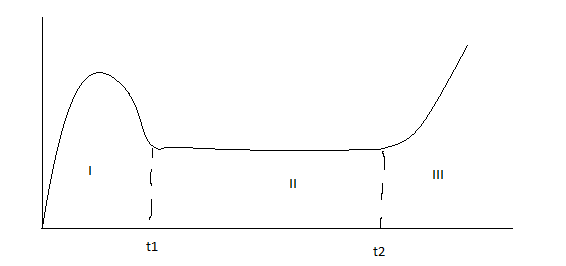
\includegraphics[width=0.6\textwidth]{38_Zhizn2.png}
\caption{Зависимость интенсивности отказов ЭС от времени: I - 0-t1 период приработки изделия, II - t1-t2 период эксплуатации изделия, III - t2-$\infty$ период старения и износа изделия}
\label{fig:Zhizn}
\end{figure}
В 1 периоде отказы ЭРЭ, узлов  происходят из-за: некачественного монтажа, сборки, низкой надежности элементов, контактов , проводников.
Во 2 периоде число отказов стабилизируется , но оно не равно нулю.
В 3 периоде отказы изделия происходят из-за физического старения материалов и износа ЭРЭ, имеющие необратимый характер.
Для нахождения р(t) = F[$\lambda$(t)] проинтегрируем $\lambda(t)$,
\begin{equation}\int_0^t \lambda (t) =- \int_0^t \frac{dp(t)}{dt} \cdot \frac{1}{p(t)} ,
\end{equation}
\begin{equation} -\int_0^t \lambda (t)dt = \int_0^t \frac{dp(t)}{p(t)}, -\int_0^t \lambda (t)dt = \ln p(t) ,
\end{equation}
\begin{equation}
p(t) = e^{- \int_{0}^{t} \lambda(t)dt}
\end{equation}

Вероятность безотказной работы имеет экспоненциальный вид, аналогично может быть найдена условная вероятность безотказной работы за интервал времени (t1,t2)
\item \underline{5)	Средняя наработка до отказа}
Tcp(t) – время работы изделия до первого отказа.
\begin{equation}
T_{cp} (t)= \int_0^\infty p(t)dt,
\end{equation}
Статистически оно находится
\begin{equation}
T^{*}_{cp} (t) = \frac{1}{N_0} \sum_{i=1}^{N_0} t_i,
\end{equation}
где $t_i$ – время работы до отказа i-го однотипного изделия.
Рассмотрим расчет показателей надежности ЭС для 2 периода $ \lambda(t)=const = \lambda$
\begin{equation}
p(t)= e^{- \lambda t},
\end{equation}
\begin{equation}
T_{cp}(t) = \int_0^\infty p(t)dt= \int_0^\infty e^{- \lambda t}dt = \frac{1}{\lambda},
\end{equation}
Рассмотренные показатели надежности справедливы для невосстанавливаемых ЭС.
\end{enumerate}

\quest{Последовательная модель надежности ЭС.}
%Вопрос №39

При последовательном соединении элементов расчет надежности производят по формуле %formula

 \begin{equation}
 P_A(t) = {\prod_{i=1}^{m}p_i(t) }
 \end{equation}
Для большего значения вероятности безотказной работы каждый элемент должен иметь значение вероятности безотказной работы близкой к единице.\\
$P_A(t)\leqslant1$,
 при увеличении количества компонентов в ЭС надежность его падает.(пример)
В тех случаях , когда нужна высокая надежность ЭС, а элементы имеют небольшое значения вероятности безотказной работы, применяют метод резервирования.

\quest{Параллельная модель надежности ЭС.}
%Вопрос №40

При параллельном соединении элементов расчет надежности производят по формуле 
 \begin{equation}
 P_A(t) = {1- \prod_{i=1}^{m}[1-p_i(t)] }
 \end{equation}
\quest{Основные этапы автоматизации:  их характеристики и особенности}
\quest{Назначение, классификация и области применения роботов}
\quest{Манипуляционные роботы: типы, характеристики, применение}
\quest{Структура механизмов манипуляционных роботов и характеристики их геометрических свойств}
\quest{Приводы манипуляторов и роботов: классификация, особенности применения}
\quest{Конструкции схватов промышленных роботов, особенности применения}
\quest{Проектирование  архитектуры интегрированной компьютерной системы управления }
\quest{Описание технологического процесса как объекта автоматизированного управления }
\quest{Описание производственного процесса как объекта автоматизированного управления: реализация АРМ различных уровней}
\quest{Выбор датчиков технологического процесса: типы измерительных устройств,  подключение.}
\quest{Теорема Котельникова (теорема отсчетов). Квазидетерминированные сигналы.}
\quest{Преобразование измерительных сигналов. Виды модуляций.}
\quest{Цифровые частотомеры.}
\quest{Цифровые фазометры.}
\quest{Цифровые вольтметры временного преобразования.}
\quest{Микропроцессорные цифровые измерительные преобразователи.}
\quest{Резистивные датчики (реостатные, пьезорезистивные).}
\quest{Электромагнитные датчики (индуктивные, трансформаторные, магнитоупругие).}
\quest{Пьезоэлектрические датчики.}
\quest{Тепловые датчики (термопары, термометры сопротивления).}
\quest{Организация и этапы разработки конструкторских документов.}
\quest{Виды КД.}
\quest{Стандартизация и БНК.}
\quest{Виды и типы схем, обозначения по ЕСКД.}
\quest{Методы компоновки конструкции ЭВС.}
\quest{Климатические зоны и категории исполнения.}
\quest{Способы защиты ЭВС от влаги.}
\quest{Защита ЭВС от механических воздействий.}
\quest{Способы обеспечения теплового режима ЭВС.}
\quest{Электромагнитные воздействия. Виды экранов.}
\quest{Виды линий связи.}
\quest{Особенности конструирования бортовых ЭВС.}
\quest{Особенности конструкций персональных ЭВМ.}
\quest{Унификация. Разновидности стандартизации.}
\quest{Требования к трассировке ПП и электрическим соединениям.}
\quest{Электромонтажные провода. Припои и флюсы.}
\quest{Волоконно-оптические линии связи (ВОЛС). Примеры использования.}
\quest{Эргономические требования к пультам, органам управления и сигнализации.}
\quest{Эргономика конструирования лицевой панели прибора.}
\quest{Защита ЭС от воздействий радиации.}
\quest{Производственный и технологический процесс и их составляющие.}
\quest{Исходные данные для разработки технологических процессов. Основные этапы разработки единичного технологического процесса.}
\quest{Требования к оформлению технологической документации. Примеры записи технологических операций.}
\quest{Основные методы изготовления печатных плат и их особенности.}
\quest{Конструктивно-технологические разновидности радиоэлектронных узлов и их сопоставительный анализ.}
\quest{Основные технологические операции при изготовлении радиоэлектронных узлов с монтажом на поверхность.}
\quest{Нанесение паяльной пасты и клея и используемое при этом оборудование.}
\quest{Принципы организации работы сборочных автоматов.}
\quest{Особенности выполнения пайки при изготовлении электронных модулей (пайка оплавлением, волной припоя, селективная пайка).}
\quest{Особенности выполнения ремонтных работ: демонтаж и монтаж компонентов.}
\quest{Материалы, используемые в технологии монтажа на поверхность.}
\quest{Виды соединительных операций при сборке.}
\quest{Соединение сваркой: разновидности, области применения.}
\quest{Соединение пайкой: разновидности, области применения, примеряя выполнения паяных соединений.}
\quest{Разработка схемы сборки изделий.}
\quest{Нормирование затрат времени при проектировании технологических процессов (штучное и подготовительно-заключительное время, определение такта и ритма выпуска изделий).}
\quest{Изготовление деталей ЭС методом литья.}
\quest{Разделительные и формообразующие операции холодной штамповки.}
\quest{Общая характеристика методов формообразования материалов и деталей при производстве ЭС.}
\quest{Изготовление электронных модулей по технологии внутреннего монтажа.}

% Вопрос 101 --------------------------------------------------------
\quest{Приведите структуру контроллера (микроЭВМ) с раздельными шинами адрес/данные и следующим составом: ХХ кб, ПЗУ – ХХ кб, индикация – 1, порты ввода/вывода – Х клавиатура – 1. Распределите адресное пространство для контроллера. Приведите таблицу распределения адресов.}

\begin{figure}[H]
\centering
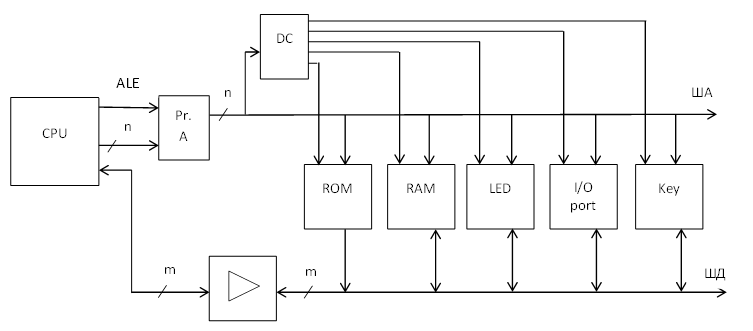
\includegraphics[width=0.8\textwidth]{101_struct.png}
\end{figure}

Допустим шина адреса процессора включает 16 бит, а шина данных – 8 бит, тогда максимальный объем адресуемой памяти составит 64 Кбайт. Предположим что для ОЗУ необходимо выделить 32 Кбайта, ПЗУ – 8 Кбайт, индикация – 256 байт, порт ввода/вывода – 256 байт, клавиатура – 256 байт. При делении адресного пространства между блоками необходимо соблюдать, чтобы начальный адрес каждого блока начинался с нулей, а старший заканчивался на “F”.

\begin{center}
\begin{tabular}{|c|c|c|}
\hline 4000h - AFFFh & ОЗУ                 &  32 Кбайт  \\
\hline 3200h - 32FFh & порт ввода/вывода   &  256 байт  \\
\hline 3100h - 31FFh & клавиатура          & 256 байт   \\
\hline 3000h - 30FFh & индикация           & 256 байт   \\
\hline 1000h - 2FFFh & ПЗУ                 &  8 Кбайт   \\
\hline 0000h - 0FFFh & регистры процессора & 4 Кбайт    \\
\hline
\end{tabular}
\end{center} 

% Вопрос 102 --------------------------------------------------------
\quest{Укажите место на структурной схеме ЭВМ различных интерфейсов. Как объединять ЭВМ в  систему? Какие условия следует выполнить при  передаче данных? Обоснуйте.}
\begin{figure}[H]
\centering
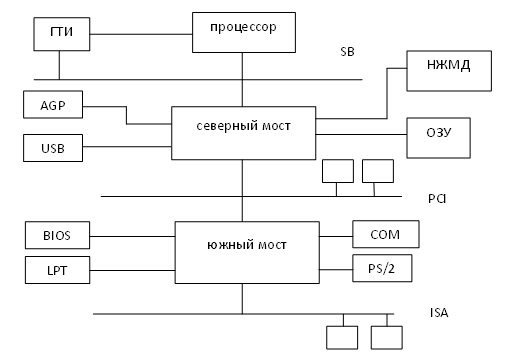
\includegraphics[width=0.8\textwidth]{./images/102_interface.png}
\end{figure}

В структуре ЭВМ в зависимости от назначения используются следующие интерфейсы:
\begin{enumerate}
\item Межпроцессорные интерфейсы – для объединения нескольких процессоров: шинный интерфейс с адресным арбитражем(по командам).
\item Межсистемный интерфейс – для объединения нескольких вычислительных блоков в одну систему. Задача возникает в кластерах. Необходим быстрый \item коммутатор и сеть типа 1 Гбит.
\item Системные интерфейсы – набор шин с правилами обмена между основными блоками ЭВМ.
\item Интерфейсы ВУ (периферийные) – обмен информации между системным блоком и ВУ.
\item Территориальные – связь с ВУ за корпусом ЭВМ, либо с внешними устройствами встроенными в корпус.(COM, USB, LPT, PS/2).
\end{enumerate}

При проектировании и реализации схемы интерфейса необходимо выполнить три условия согласования для передачи от устройства к приемнику:
\begin{enumerate}
\item Механические
\item Логические
\item Электрические
\end{enumerate}

Механические --- тип разъема, число контактов, расстояние между ними.

Логические --- последовательность передачи сигналов и наличие сигналов синхронизации определяется протоколом интерфейса, форматом передаваемого кадра и в конечном счете программным управлением. Уровни <<1>> и <<0>> так же определяются логическими условиями.

Электрические --- временные положения импульсов, величина фронтов, длительность сигналов синхронизации, фазовые сдвиги.

Помимо условий согласования необходимо выполнить интерфейсные функции: на время в буфере сохранить сигнал, проанализировать ответный сигнал, сформировать сигнал сопровождения и т.д..

% Вопрос 103 --------------------------------------------------------
\quest{Расставьте по убыванию значимости параметры ЭВМ по критерию производительности. Охарактеризуйте эти параметры.}

Производительность – число операций выполняемых в единицу времени. Если данные представлены в целом коде – единица измерения MIPS (миллион инструкций в секунду). Если данные представлены в  формате ПЗ – единица измерения FLOP (операций в секунду). Производительность комьютера не вычислияется, а определяется в процессе тестирования по скорости выполения определенных операций в программной среде.
Параметры влияющие на производительность ЭВМ: 
\begin{enumerate}
\item Операционные ресурсы
\item Емкость памяти ресурсы
\item Разрядность шины адреса и данных
\item Быстродействие
\item Память
\end{enumerate}

Операционные ресурсы – это перечень действий, которые может делать (выполнять) аппаратура ВС в плане обработки информации (исходных данных). В этот перечень прежде всего включается система машинных операций – список F=\{+,-,*,/,…\}. Кроме того, это порождающая ее (систему операций) система машинных команд К=\{К1, …, КN\}. В понятие операционные ресурсы включаются также способы представления информации в ЭВМ, способы представления чисел, текстов, логических значений. Чем шире перечень действий, чем шире многообразие способов представления данных – тем шире операционные ресурсы ЭВМ и, следовательно, возможности ВС в плане обработки информации.

Емкость памяти – очевидная техническая характеристика, которая характеризует вместимость хранилища программ и данных ВС. Единицы измерения – бит,  байт,  килобайт , мегабайт,  гигабайт, терабайт.  Емкость  памяти $ E $ обычно  кратна степени 2: $ E = 2^{m}$, $ m $ – длина (разрядность) адреса.

Разрядность шины адреса и данных – определяет количество бит передаваемых шиной. Чем больше разрядность, тем большее количество информации можно передать за один такт.

Быстродействие – это характеристика, которая отвечает на вопрос, как быстро действует (работает) аппаратура ЭВМ. Эта характеристика определяет потенциальные возможности устройств, указывает на верхнюю границу. Относится к отдельным устройствам, а не ВС в целом. Так, быстродействие процессора характеризует скорость, с которой это устройство может выполнять операции: Быстродействие определяется количеством операций в единицу времени и зависит от времени выполнения операции: $ V=1/t $ – чем меньше время выполнения операции t, тем выше быстродействие. Быстродействие процессора определяется временем выполнения команд. Память ЭВМ предназначена для хранения, записи и чтения информации. Быстродействие памяти принято характеризовать количеством операций чтения/записи в единицу времени. Память ЭВМ строится на базе ЗУ (БИС ОЗУ, ППЗУ). Быстродействие памяти зависит от быстродействия ЗУ и ее внутренней организации. 

% Вопрос 104 --------------------------------------------------------
\quest{Преобразуйте десятичное число в различные форматы хранения. В какой форме хранятся в памяти ЭВМ символы. Приведите два примера.}

Методика преобразования целых десятичных чисел в двоичные коды различна в зависимости от знака числа.

Положительные числа имеют одинаковое представление в обратном, прямом и дополнительном кодах, и имеют цифру $ 0 $ в знаковом разряде: $ 127_{10}=01111111_{2} $.

Отрицательные числа представляются в виде дополнительного кода. Преобразование из прямого кода в дополнительный сводится к следующим действиям:
\begin{enumerate}
\item Прямой код

В знаковый разряд помещается цифра $ 1 $, а в разряды цифровой части числа – двоичный код абсолютной величины: $ -127_{10}=11111111_{2} $
\item Обратный код

Получается инвертированием всех цифр двоичного кода без учета знакового разряда: нули заменяются единицами и наоборот: $ -127_{10}=10000000_{2} $
\item Дополнительный код

К обратному коду добавляется единица к младшему разряду: $ -127_{10}=10000001_{2} $.
Дополнительный код и есть представление отрицательного числа $ -127 $.
\end{enumerate}  

Преобразование вещественных чисел со знаком:

Вещественное число $ X $ можно представить в виде произведения мантиссы $ m $ и основания системы счисления $ q $ в некоторой степени $ n $ : $ X=m \ast q^{n} $. 
Например: $ 25.324 = 0.25324\ast 10^{2} $. Здесь $ 0.25324 $ – нормализовання мантисса, $ 2 $ – порядок(степень). Порядок указывает, на какое количество позиций должна сместиться запятая в мантиссе. Необходимо, чтобы значение мантиссы было нормализованно и удовлетворяло условию: $ 0.5 \leq m < 1 $. Другими словами нормализованная мантисса меньше $ 1 $ и первая значащая цифра после запятой не меньше $ 5 $. 
Двоичный код вещественного числа должен быть следующего формата:

\begin{center}
\begin{tabular}{|c|c|c|}
\hline 8 бит   & 1 бит & 23 бит   \\ 
\hline порядок & знак  & мантисса \\ 
\hline 
\end{tabular}
\end{center}
 
Допустим имеем число $ 278.15 $, переведем его в двоичный код в формате п.з.. Подставим это число в формулу $ X=m\ast q^{n} $. Получим уравнение:$ 278.15= m\ast q^{n} $. Для нахождения мантиссы $ m $ неизвестен порядок $ n $, найдем его: $ 2^{8}=256 $, что меньше $ 278.15 $, возьмем следующую степень по порядку $ -2^{9}=512 $. В данном случае $ 512>278.15 $, по этому выберем $ q^{n}=2^{9} $. Тогда мантисса $ m=X/q^{n} = 278.15 / 512 = 0.543 $. Прямой код мантиссы $ m = 0.543 = 10001_{2} $. Прямой код порядка $ n=9=1001_{2} $. Теперь можно записать число в формате с плавающей запятой:

\begin{center}
\begin{tabular}{|c|c|c|}
\hline порядок  & знак & мантисса                \\ 
\hline 00001001 & 0    & 10001000000000000000000 \\ 
\hline 
\end{tabular}
\end{center}

Преобразование в шестнадцатеричные коды:

Преобразование из двоичного кода в шестнадцатеричный производят в два этапа: перевод в двоичный код, а затем уже в шестнадцатеричный.

Для преобразования из двоичного кода в шестнадцатеричный нужно условно разбить код на тетрады. Например, необходимо преобразовать код: $ 110100011,1111_{2} $. Разбиваем его на тетрады: $ 1 \mid 1010 \mid 0011 \mid 1111 $. И каждую тетраду заменяем на соответствующее шестнадцатеричное число. $ 1_{2} = 1_{16} $, $ 1010_{2} = A_{16} $, $ 0011_{2} = 3_{16} $, $ 1111_{2} = F_{16} $. В итоге получим число $ 1A3,F $. В таблице указано соответствие двоичных чисел шестнадцатеричным:

\begin{center}
\small
\begin{tabular}{|c|c|c|c|c|c|c|c|c|c|c|c|c|c|c|c|}
\hline 0000 & 0001 & 0010 & 0011 & 0100 & 0101 & 0110 & 0111 & 1000 & 1001 & 1010 & 1011 & 1100 & 1101 & 1110 & 1111 \\ 
\hline 0 & 1 & 2 & 3 & 4 & 5 & 6 & 7 & 8 & 9 & A & B & C & D & E & F \\ 
\hline 
\end{tabular}
\end{center}

Преобразование в двоично-десятичный код:

Преобразование десятичного числа в двоично-десятичный код осуществляется переводом каждого разряда десятичного числа в соответствующий четырехбитовый эквивалент. Например, число $ 311_{10} = 011100010001_{BCD} $. Здесь  $3_{10} = 0111_{2}$, $1_{10} = 0001_{2}$.

Хранение символов в ЭВМ:

Каждая буква принадлежит определенному алфавиту, в котором символы следуют друг за другом и, следовательно, могут быть пронумерованы последовательными целыми числами. Каждой букве можно сопоставить целое положительное число и назвать его кодом символа. Именно этот код будет храниться в памяти компьютера, а при выводе на экран или бумагу «преобразовываться» в соответствующий ему символ. Чтобы отличить представление чисел от представления символов в памяти компьютера, приходится также хранить информацию о том, какие именно данные закодированы в конкретной области памяти.

Соответствие букв определенного алфавита с числами-кодами формирует так называемую таблицу кодирования. Другими словами, каждый символ конкретного алфавита имеет свой числовой код в соответствии с определенной таблицей кодирования. Американским национальным институтом стандартизации (ANSI) была разработана таблица кодирования символов, которая впоследствии была использована во всех операционных системах. Эта таблица называется ASCII.

Например, символу $A$ соответсвует код 41h, а символу $+$ код 2Bh. 

% Вопрос 105 --------------------------------------------------------
\quest{Сопоставьте принципы печати лазерного и струйного принтеров, опишите и сравните их.}

{\bf Лазерный принтер:}

В основе печати лазерным способом лежит принцип переноса изображения из кодов на образующую фотобарабана лазерным лучом. Луч двигается слева направо(принцип монитора) при этом модулируется так же знакогенераторм или графическим процессором, барабан перемещается всякий раз на одну линию и далее уже красящее вещество с барабана механически переносится на бумагу. Печатающий узел называется катридж. Основа в катридже - кожух с продольным отверстием, которое закрывается шторкой. При сдвиге шторки через отверстие виден барабан светлого света, покрытый селеном потому, что он под воздействием света проявляет внешний фотоэлектрический эффект. Помимо барабана в кожухе размещается красящий порошок - тонер - мелкодисперсный синтетический состав, плавящийся при нагревании. С торцов катриджа система шестерен для управления вращением барабана. Так же в катридже расположен электрод, на который подается высокое отрицательное напряжение. Коды символов, поступая в процессор принтера преобразовываются в управляющую последовательность кодов. Эта последовательность единиц и нулей посылается на лазер - источник света с тонким лучом. Луч направлен на зеркало, которое перемещает его строго по образующей барабана с одного конца на другой. Подавая 1 и 0 на лазер, формируются светлые и темные точки на образующей цилиндра.
\begin{figure}[H]
\centering
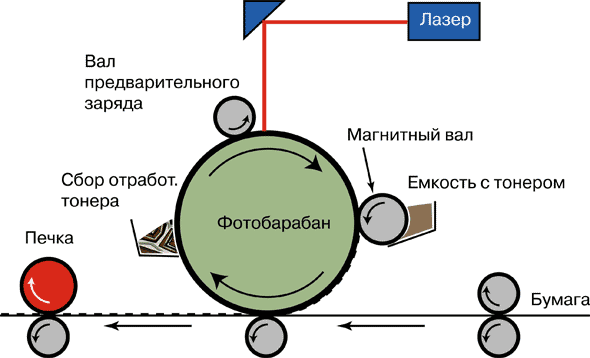
\includegraphics[width=0.3\textwidth]{/105_Laser.png}
\caption{Лазерный принтер}
\end{figure}
В начальном состоянии барабан не заряжен, тонера на нем нет. Но рядом с барабаном имеется электрод, заряжающий барабан отрицательно. При вращении барабана его поверхность заряжается равномерно. При печати луч лазера попадает через зеркало на образующую барабана и выбивает электроны в том месте куда он попал. После того как пройдет развертка, формируются заряженные и незаряженные точечки. При дальнейшем движении сверху сыплется порошок, имеющий отрицательный заряд. При соприкосновении с поверхностью цилиндра порошок прилипает к его незаряженным частям. Барабан вращается дальше, и в нижней точке соприкасается с листом бумаги, образуя оттиск на бумаге - барабан вдавливается в бумагу. Бумага двигается далее по роликам нагревается, и, порошок расплавляясь, въедается в бумагу. Поскольку развертка движется периодически, на поверхности барабана получаем рисунок, символы в котором непрерывным путем переносятся на бумагу.

Преимущество: скорость печатания лазерных принтеров велика - до нескольких десятков страниц в минуту. Разрешающая способность 300-1200 dpi. Являются экономичными.

Недостаток: один тонер. поэтому для цветной печати выполняют три пишущих узла, с разными тонерами (RGB). Цвета наносятся друг за другом  и затем сплавляются. 

{\bf Струйный принтер:}

Развитием в сторону бесконтактного способа матричной печати (иголок), является печать капельками жидкости - струйные принтеры. У таких принтеров капельки красящего вещества выстреливают из сопла головки, пролетают небольшое расстояние и попадают на бумагу. Основная проблема в таких устройствах печтаи - это то, как "прилепить" каплю жидкости к бумаге. В струйных принтерах бумага должна быть не очень плотной, и в то же время иметь плотность не хуже некоторого значения, по скольку жидкость распространяется во все стороны. Задача решается совместно: определенное качество бумаги и текучести чернил. По скольку капелька вытекает из сопла, то можно размещая по три сопла рядом печатать цветом. На практике существуют два способа струйной печати: {\sl Непрерывная и импульсная струйная печать.}

{\sl Непрерывная струйная печать:}

Чернила подаются в печатающую головку с помощью насоса. Возникающая под создаваемым им давлением струя разбивается на капельки за счет вибрации, вызываемой, например, пьезоэлектрическим элементом. Разумеется, до бумаги должны долететь не все, а только часть капелек, иначе никакого изображения не получится - бумага просто будет равномерно залита чернилами.
Вылетая из сопла, капельки проскакивают через заряжающий электрод. Получив электрический заряд, они попадают в поле отклоняющего электрода, на который подается высокое напряжение. Изменяя напряжение на отклоняющем электроде, можно заставить капельки поменять траекторию полета. Если состоящая из заряженных капелек струя не отклоняется в сторону, она попадает в уловитель, из которого неиспользованные чернила стекают в накопитель, проходят стадию удаления воздушных пузырьков (дегазации) и снова сливаются в основной резервуар с краской.
Сменившие направление полета под действием электрического поля отклоняющего электрода капельки попадают на бумагу, формируя на ней изображение. Угол отклонения траектории зависит от того, насколько сильно изменяется напряжение.
Системы непрерывной струйной печати отличаются тем, что в них применяется дорогая электропроводная краска, способная получить заряд. Так как между соплом и бумагой необходимо разместить два электрода, увеличивается дальность полета капелек и, следовательно, им необходимо придать большую начальную скорость. Очень высока и производительность сопел печатающей головки - из них в секунду вылетает от 50 до 150 тысяч капелек. Однако сам процесс печати не назовешь очень быстрым.

Недостаток: медленная печать, серьезные эксплуатационные расходы, обусловленные дороговизной чернил и сложностью обслуживания таких принтеров, и, конечно, немалая цена самого оборудования.

Преимущество: высокое качество получаемых с ее помощью цветных изображений.

{\sl Импульсная струйная печать:}

Капельки из сопел пьезоэлектрической головки вылетают под воздействием создаваемого на очень короткое время избыточного давления в камере с чернилами. Для образования в камере избыточного давления применяется диск из пьезоэлектрика. Когда к нему подводится напряжение, он деформируется (изгибается). Выгнувшись, диск, который служит одной из стенок камеры с чернилами, резко уменьшает ее объем, оказавшиеся лишними чернила вылетают при этом из сопла в виде капельки. Для заполнения камеры, когда напряжение снято и пьезоэлектрический диск возвращается к исходной форме, применяется капиллярный способ подачи чернил из резервуара. Конструкция современных пузырьковых головок допускает использование быстро сохнущих чернил, благодаря чему капельки не успевают впитаться в бумагу или растечься - они просто моментально высыхают. Благодаря увеличению скорости, с которой из сопел выстреливаются капельки, можно увеличить зазор между головкой и бумагой. Больший зазор позволяет применять бумагу худшего качества, неровную или более плотную.Такая технология привела к упрощению конструкции, удешевлению самих принтеров, так и к снижению эксплуатационных затрат.               

\quest{Приведите две схемы подключения клавиатуры к портам ввода-вывода. Приведите алгоритм опроса пассивной матричной клавиатуры.}
\quest{Выберите способ обмена данными между процессором и внешним устройством. Обоснуйте выбор. Напишите процедуру ввода или вывода данных в память ЭВМ в мнемонике команд (уровень ассемблера).}
\quest{Приведите основные архитектурные варианта построения операционных систем. Поясните понятие <<виртуальная машина>>.}
\quest{Спроектировать устройство управления программного типа. Число микрокоманд в цикле – не более 7. Привести примеры циклов: выборка команды, чтение памяти и запись в память. Чем определяется период следования тактового сигнала.}
\quest{Спроектировать устройство микропрограммного управления автономного типа. Источник управляющих кодов – счетчик микрокоманд, число состояний счетчика – 32. Разрядность регистра микрокоманд – 24.}
\quest{Привести примеры процедур с различными способами адресации для пересылки содержимого ячейки памяти команд в ячейку памяти данных в мнемонике команд, адресация в пределах одной страницы (64 кб). Пояснить необходимость модификации адресов для доступа к данным и возможные их способы.}
\quest{Прерывания как способ изменения адреса в управляющей команде. Привести пример системы прерывания. Описать процедуру опознавания запроса на прерывание с маскированием.}
\quest{Системы памяти ЭВМ. Назначение каждого типа элементов памяти и место его в иерархии. Что дает для характеристик ЭВМ каждый тип элементов памяти.}
\quest{Память программ. Виды носителей. Жесткие диски и их твердотельные аналоги.}
\quest{Компиляторы. Назначение компиляторов, их виды. Последовательность процедуры компиляции.}

% Вопрос 116 ----------------------------------------------------------
\quest{Контроль информации при последовательной передаче двоичного кода. Методы контроля. Контроль передачи информации при обмене словами (байтами). Методы.}

Считается, что цифровая техника обеспечивает безошибочные вычисления, так как информация представлена однозначно в виде 0 и 1, в отличие от аналоговых схем, где носителем информации является уровень сигнала, который может меняться. Однако, при передаче и хранении информации возможно ее искажение, поэтому вводятся средства контроля, цель которых - не остановить вычисления, а получить результат с максимальной достоверностью.

Контроль проводится как аппаратными средствами, так и программными. Аппаратные средства включаются в состав функциональных блоков процессора, контроллера ввода/вывода, средств передачи. Программно контролируются память, выполнение отдельных операций.
Назначение всех средств контроля можно разделить на контроль передачи информации и контроль преобразования.

\begin{center}
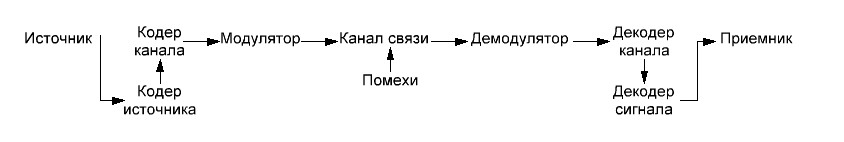
\includegraphics[width=0.9\textwidth]{116_Channel.png}\\
\end{center}
Для повышения помехоустойчивости к передаваемому коду добавляют доп. разряды, при этом число возможных состояний кода увеличивается, однако число информативных состояний остается прежним. То есть часть состояний - запрещенные. Кодовое расстояние - число разрядов из всей совокупности передаваемых кодов, в которых 1 и 0 не совпадают.

Простейшие коды:
\begin{enumerate}
\item добавление контрольного разряда - контроль четности. Двойные ошибки не замечаются, исправление информации невозможно - только контроль правильности.
\item Коды Хэмминга. Кодовое расстояние - 3. Позволяют выявить и исправить одиночную ошибку. Получаются путем объединения по XOR части разрядов числа, но несколько раз.
\item Простой повтор нечетное число раз - по большинству.
\end{enumerate}

При передаче файлами применяется контроль с помощью СRC-кода. Суть: после передачи файла к нему прицепляется контрольная последовательность, получаемая как остаток от деления значения файла на определенный полином, известный и приемнику, и источнику. Полином выбран так, что его значение в квадрате меньше максимального значения файла. Приемник, зная полином, вычисляет свой CRC и сравнивает его с полученным от источника. Если совпадают - передача правильная. Если нет - запрашивается повтор передачи.

Метод наибольшего правдоподобия - по алгоритму Виттерби. Он при приеме предусматривает некоторые ожидаемые стандартные комбинации. В настоящее время применяется в системах цифровой связи.

% Вопрос 117 ----------------------------------------------------------
\quest{Приведите основные структуры объединения процессоров в многопроцессорных системах. В чем суть ограничений архитектуры Фон-Неймана.}

Для архитектуры фон Неймана характерны следующие свойства:
\begin{enumerate}
\item единый процессор и единая память
\item линейная организация памяти
\item команды низкого уровня
\item любая операция предусматривает чтение памяти команд, и только затем - обращение к памяти данных. Связь процессора с памятью по ША и ШД.
\end{enumerate}

Реальные проводники из-за своих паразитных характеристик не позволяют передавать сигналы с высокой скоростью, поэтому увеличение производительности за счет повышения тактовой частоты уже почти невозможно. Таким образом, нужны новые структуры ЭВМ.
\begin{enumerate}
\item конвейерная – ряд процессоров, специализированных под конкретные операции, выполняют операции последовательно, передавая результат друг другу. За счет этого может выполняться одновременное преобразование нескольких слов данных. Конвейер реализуется на кристалле, т.к. отдельные блоки объединять накладно.
\item параллельная - объединение нескольких машин через канал. Канал - узкое место. Например, двухмашинный комплекс, в котором вторая машина работает в качестве горячего резерва.
\item иерархическая - один из процессоров выделяется как главный, вспомогательный подключается через блок сопряжения, но при этом теряется универсальность.
\end{enumerate}

Векторно-конвейерные суперкомпьютеры. Конвейер, как последовательное включение процессорных блоков, сохраняется, однако каждый процессорный блок обрабатывает не одно слово данных, а вектор - несколько составленных вместе слов, т.е. в структуре ЭВМ имеются параллельные каналы обработки, соединенные в конвейер. Основная идея - распараллеливание циклического процесса.

Симметричные (SMP) системы - системы с общей памятью. Подключение нескольких процессоров к общей памяти, каждому процессору выделяется буферная память. При этом пока один процессор занимает шину, остальные могут работать с информацией из кэша. С ростом числа процессоров эффективность метода падает, т.к. приходится постоянно наполнять кэш. Замена шины на электронный коммутатор позволяет увеличить скорость передачи и организовать уже несколько одновременных процессов обращения к памяти. 

Структуры с массовым параллелизмом (MPP) - предельный случай SMP, когда каждому процессору выделен свой блок памяти. В структуре те же блоки, но компоновка иная. Например, обмен информацией происходит по пути: память 1 -> кэш 1-го проц. -> коммутатор -> кэш 2-го проц. -> память 2. Раздельная память увеличивает интенсивность обмена процессора со своей памятью, и лишь малое время уходит на обмен между блоками памяти разных процессоров, как правило - после выполнения каких-либо законченных процедур.

\begin{center}
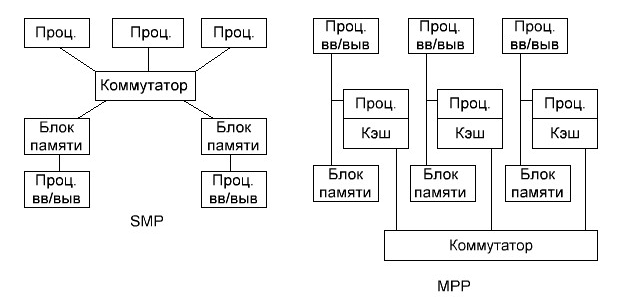
\includegraphics[width=0.8\textwidth]{117_SMP_MPP.png}\\
\end{center}
Кластеры - объединение в единое вычислительное пространство самостоятельных ВС по быстрым сетям. В кластере должен быть управляющий блок - аналог сетевого сервера, по скорости значительно превосходящий остальные узлы. Его задача - распределение и контроль информации.

% Вопрос 118 ----------------------------------------------------------
\quest{Сравните структуры двух МПК, имеющих организацию SMP и MPP. Приведите их структурные схемы.}

Симметричные (SMP) системы - системы с общей памятью. Подключение нескольких процессоров к общей памяти требует подключения их к общим шинам адреса и данных. При параллельном подключении процессоров к шине доступ к памяти разрешен только одному - это не увеличивает производительность, поэтому каждому процессору выделяется буферная память. При этом пока один процессор занимает шину, остальные могут работать с информацией из кэша. С ростом числа процессоров эффективность метода падает, т.к. приходится постоянно наполнять кэш. Замена шины на электронный коммутатор позволяет увеличить скорость передачи и организовать уже несколько одновременных процессов обращения к памяти. Адресное пространство для всех общее, но оно распределено по некольким модулям. Каждый процессор преимущественно работает со своим модулем, но может обратиться и к любому другому. Внешние устройства подключаются к блоку памяти или коммутатору через специальные каналы - процессоры ввода/вывода.

Пример SMP системы – "МВК Эльбрус". Общее число процессоров – до 10. Память разделена на 2 логических блока, но адресное пространство общее. Выделяется один управляющий процессор. Развитая система вв\textbackslash выв, так как комплекс должен обслуживать технологическое оборудование.

\begin{center}
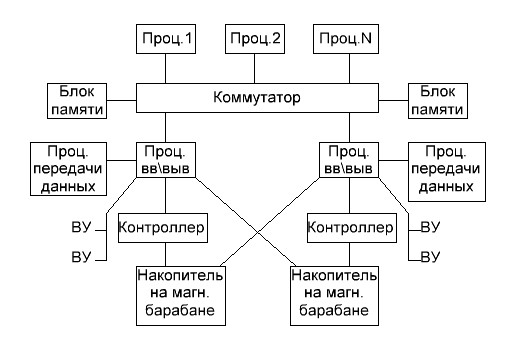
\includegraphics[width=0.7\textwidth]{118_Elbrus.png}
\end{center}
Структуры с массовым параллелизмом (MPP) - предельный случай SMP, когда каждому процессору выделен свой блок памяти. В структуре те же блоки, но компоновка иная. Например, обмен информацией происходит по пути: память 1 ->кэш 1-го проц.->коммутатор->кэш 2-го проц.-> память 2. Раздельная память увеличивает интенсивность обмена процессора со своей памятью, и лишь малое время уходит на обмен между блоками памяти разных процессоров, как правило - после выполнения каких-либо законченных процедур.

С ростом числа процессоров растет сложность коммутаторов. Простейшая структура - матрица. Сложнее - цилиндр, затем - тор (он же - "куб"), соединение кубов - "гиперкуб".

Пример MPP – структуры – МВС-1000. Система 3-го поколения. Размещается в стойках промышленного стандарта. Всего 768 процессоров (по 64 в стойке). В состав системы входят управляющая ЭВМ, файл-сервер, сеть межпроцессорного обмена и FastEthernet. Обязательно – система контроля питания. Коммутатор – двумерный тор.

\begin{center}
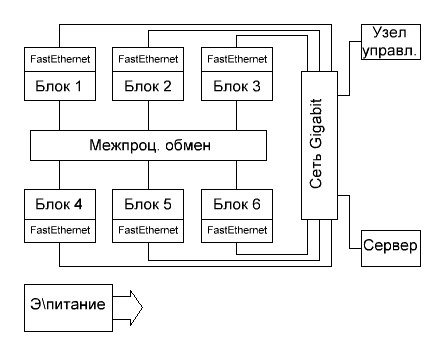
\includegraphics[width=0.7\textwidth]{118_MBC-1000.png}
\end{center}
% Вопрос 119 ----------------------------------------------------------
\quest{Сравните характеристики двух последовательных интерфейсов RS-232С и USB. Приведите  структурную организацию интерфейсов и формат передаваемых данных.}

RS-232C – последовательная передача по байтам. Формат передачи: стартовый сигнал (1,5-2 такта), 8 разрядов данных от младшего к старшему со строго определенной заранее скоростью, затем контрольный разряд, затем стоповый сигнал и небольшая пауза. Скорости: 2400, 4800, 9600, 19200, 38400.

Для двустороннего обмена достаточно трех проводников – TXD, RXD, GND. Кабель перекручен (TXD источника подключается к RXD приемника, и наоборот). Разъемы COM-порта – DB-25, DB-9. Помимо информационных сигналов, через разъем посылаются сигналы сопровождения – ошибка, готовность.

Интерфейс потенциальный, уровни 0 и 1 передаются уровнями напряжения ±5…15 В. Максимальная длина кабеля – 1,4…1,7 м.

USB – последовательный цепочечный интерфейс с обменом файлами. Частота – 33,6 МГц. Сигналы на линиях – дифференциальные, то есть сигнал распространяется токовый. Размах - ±4 В при питании 5 В. Интерфейс реализуется микросхемой-адаптером с буферной памятью. Обмен между ней и процессором идет с временем цикла процессора, а передача всегда с фиксированной скоростью, то есть для нее нужен собственный тактовый генератор. Время передачи файла соизмеримо с передачей 1 бита по COM-порту. Плата за  скорость - аппаратная часть.

Формат кадра:
\begin{itemize}
\item стартовый импульс
\item адресная часть – 7 бит, адресует до 127 устройств.
\item биты передаваемой информации – число фиксированное, зависит от принятого формата
\item разряды контроля – 5-7 бит – CRC-код.
\item бит конца передачи.
\end{itemize}

Таким образом, передача по кадрам асинхронная, но внутри кадра биты передаются со строго определенной скоростью. В качестве кабеля применяют витую пару (50 Ом). Длина 3…10 м (но рекомендуется не более 5).

% Вопрос 120 ----------------------------------------------------------
\quest{Какие принципы программного управления характерны для командного и микро-командного способов управления. В чем сходство и различие этих способов. Покажите на примере структурной схемы устройств управления.}

Принципы программного управления:
\begin{enumerate}
\item Информация кодируется в двоичной форме и разделяется на слова
\item Перед обработкой слова информации исходные данные размещаются в ячейках памяти ЭВМ. Ячейки памяти нумеруются – адреса.
\item Алгоритм обработки представляется в виде последовательности команд - программы. Каждая команда задает ЭВМ тип выполняемой операции и может определять местоположение операндов в памяти ЭВМ указанием  номера ячейки.
\item Команды также кодируются в двоичной форме и располагаются в ячейках памяти ЭВМ
\item Выполнение программы сводится к поочередному выбору команд из памяти ЭВМ и их выполнению. Порядок их выполнения задается алгоритмом и зависит от исходных данных
\end{enumerate}

Три уровня команд:
\begin{enumerate}
\item микрокоманды – элементарное преобразование операнда (пересылка из регистра в регистр, вывод содержимого на выход данных). Микрокоманда выполняется за один такт синхронизации. За время выполнения микрокоманды происходит фиксация входного операнда в регистре процессора (по фронту синхр.) и само преобразование операнда с фиксацией в выходном регистре (по срезу синхр.). Длительность синхросигнала должна быть достаточной для того, чтобы успели закончиться переходные процессы в комбинационных схемах и при записи в регистр.
\item команды – часто приравнивают к операциям. Команда может включать в себя до десятков микрокоманд.
\item макрокоманды (тэги) – появились в силу того, что сложные процедуры требовали большого числа команд, обращений в память. Переход к макрокомандам сокращал их число, повышая скорость выполнения.
\end{enumerate}

Устройство управления с жесткими связями.

Процессор с командным типом управления включает в себя управляющую и операционную части. На вход управляющей поступает КОП, который расшифровывается в сигналы микрокоманд. По результатам текущих операций в управляющую часть возвращаются флаги.
Дешифратор команд выполнен на ПЛМ. Сам пользователь не может изменить ее содержимое.

\begin{center}
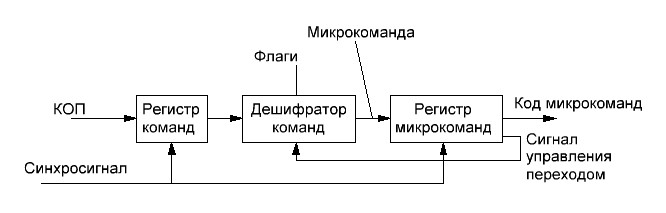
\includegraphics[width=0.8\textwidth]{120_microcom.png}
\end{center}
Устройство микропрограммного управления

В его основе лежит введение промежуточного преобразования кода команд в микрокоманды с применением схем памяти. С приходом КОП дешифратор начального адреса микрокоманды формирует адрес, по которому из памяти микрокоманд необходимо считать первую микрокоманду. Считанный код содержит признак смещения, по которому определяется адрес следующей микрокоманды. Замена содержимого памяти микрокоманд эквивалентна замене микрокоманд. Для анализа текущего состояния процессора на схему управления поступают сигналы управления – флаги.

\begin{center}
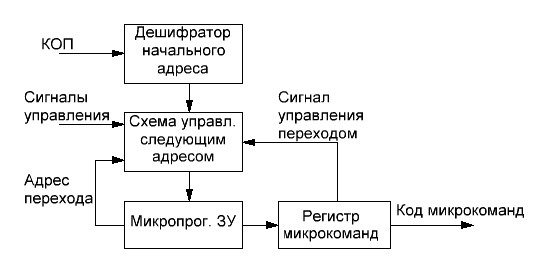
\includegraphics[width=0.8\textwidth]{120_microprog.png}
\end{center}
\quest{Основные понятия процесса проектирования систем управления. Цель процесса проектирования.}
\quest{Системный подход к проектированию.}
\quest{Структура процесса автоматизированного проектирования.}
\quest{Основные типы автоматизированных систем, разновидности САПР.}
\quest{Стадии проектирования автоматизированных систем и аспекты их описания.}
\quest{Особенности проектирования САПР.}
\quest{Понятие о CALS-технологиях.}
\quest{Открытые системы.}
\quest{Техническое обеспечение систем автоматизированного проектирования.}
\quest{Типы сетей, методы доступа в сетях, протоколы и стеки протоколов в вычислительных сетях.}
\quest{САПР систем управления.}
\quest{Автоматизация управления предприятием, логистические системы.}
\quest{АСУТП, автоматизированные системы делопроизводства.}
\quest{Математическое обеспечение анализа проектных решений.}
\quest{Компоненты математического обеспечения, структура вычислительного процесса анализа.}
\quest{Математическое обеспечение анализа на макроуровне.}
\quest{Математическое обеспечение анализа на микроуровне.}
\quest{Математическое обеспечение анализа на функционально-логическом уровне.}
\quest{Математическое обеспечение анализа на системном уровне.}
\quest{Математическое обеспечение подсистем машинной графики и геометрического моделирования.}

% Вопрос 141 --------------------------------------------------------
\quest{Схемы мультивибратора на транзисторах и ОУ.}

Мультивибратор — генератор колебаний прямоугольной формы с короткими фронтами. Мультивибратор работает в автоколебательном режиме и не имеет устойчивых состояний. По сути представляет собой двухкаскадный резистивный усилитель с глубокой положительной обратной связью. Длительность периода из двух частей равна:

\begin{displaymath}
T = t_1 + t_2 = \ln 2 \cdot R_2 C_1 + \ln 2 \cdot R_3 C_2
\end{displaymath}
\begin{figure}[H]
\centering
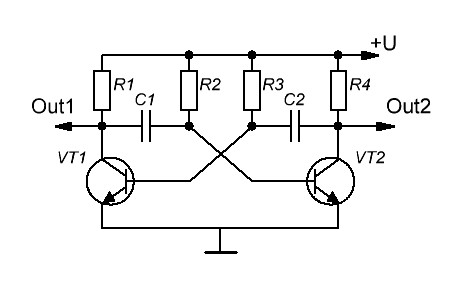
\includegraphics[width=0.4\textwidth]{141_tranz.jpg}
\caption{Мультивибратор на транзисторах}
\end{figure}
На ОУ строят мультивибраторы работающие на относительно низких частотах. Для регулировки соотношения длительности положительных и отрицательных импульсов применяется следующая схема (см. рис.).
\begin{figure}[H]
\centering
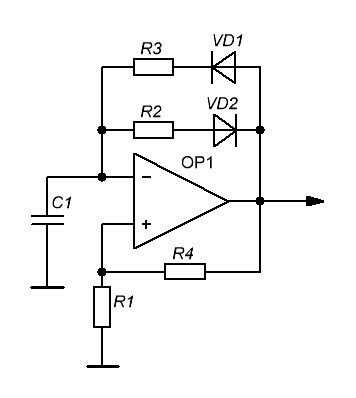
\includegraphics[width=0.35\textwidth]{141_OU_unsim.jpg}
\caption{Несимметричный мультивибратор на ОУ}
\end{figure}

Время импульса и паузы соответственно:
\begin{displaymath}
t_\text{и} = R_1 C_1 \ln (1 + 2 \frac{R_4}{R_3} )
\end{displaymath}
\begin{displaymath}
t_\text{п} = R_2 C_1 \ln (1 + 2 \frac{R_4}{R_3} )
\end{displaymath}
% Вопрос 142 --------------------------------------------------------
\quest{Схема одновибратора на транзисторах.}

Одновибратор - предназначен для формирования прямоугольных импульсов заданной длительности. Имеет одно устойчивое состояние, при котором VT1 закрыт, а VT2 открыт. Длительность генерируемого импульса $T_\text{имп} = 0,7 C_1 R_2 $.

\begin{figure}[H]
\centering
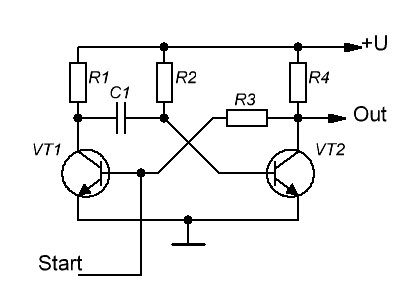
\includegraphics[width=0.4\textwidth]{142.jpg}
\caption{Одновибратор на транзисторах}
\end{figure}

% Вопрос 143 --------------------------------------------------------
\quest{Масштабный усилитель на ОУ с К=+10.}

Так как коэффициент усиления положительный, усилитель неинвертирующий:
\begin{figure}[H]
\centering
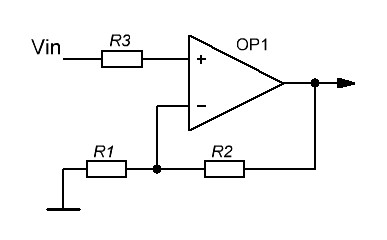
\includegraphics[width=0.4\textwidth]{143.jpg}
\caption{Масштабный усилитель}
\end{figure}
Коэффициент усиления вычисляется по формуле $K = 1 + \frac{R_2}{R_1} $. Отсюда, для получения коэффициента усиления 10 необходимо, чтобы выполнялось условие $R_2 = (K - 1) R_1 = 9 R_1$. Выбор номиналов зависит от напряжения питания и требуемых токов. Резистор R3, устанавливаемый при необходимости, уменьшает ошибку, возникающую из-за тока смещения, и имеет номинал, равный $R_1 \parallel R_2$.

% Вопрос 144 --------------------------------------------------------
\quest{Повторитель на ОУ.}
Рисовать смысла не имеет - просто ОУ со 100\% отрицательной обратной связью. Сигнал поступает на неинвертирующий вход, снимается с выхода. Выходное напряжение равно напряжению на входе, входное сопротивление от 1 MОм до 10 TОм. Повторитель применяется как буферный усилитель, для исключения влияния низкоомной нагрузки на источник с высоким выходным сопротивлением.

% Вопрос 145 --------------------------------------------------------
\quest{Двухтактный трансформаторный усилитель мощности, работающий в режиме АВ.}
Транзисторы работают поочередно, каждый во время своего полупериода входного двухполярного сигнала. Для перевода усилителя в режим АВ используются резисторы R1 и R2, создающие напряжение смещения на базах транзисторов (если бы их не было, то были бы искажения типа "ступенька", из-за использования нелинейной части характеристики транзисторов - усилитель работал бы в режиме В).
\begin{figure}[H]
\centering
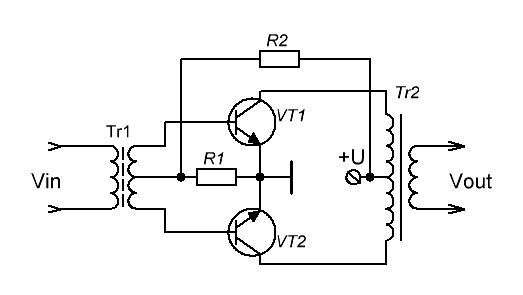
\includegraphics[width=0.6\textwidth]{145.jpg}
\caption{Двухтактный усилитель мощности}
\end{figure}

% Вопрос 146 --------------------------------------------------------
\quest{Избирательные усилители LC и RC.}

Избирательные усилители предназначены для усиления сигналов в узкой полосе частот. По принципу действия различают усилители резонансные и с обратной связью. В резонансных в качестве нагрузки используется колебательный контур, имеющий большое сопротивление на резонансной частоте и малое на остальных. Избирательные свойства оцениваются добротностью $Q = \frac{f_0}{2 \Delta f}$, где $2 \Delta f$ - полоса пропускания.
Усилители с ОС обычно используются на низких частотах. Резонансная частота такого усилителя определяется по формуле $f_0 = \frac{1}{2 \pi R C}$.
\begin{figure}[H]
\centering
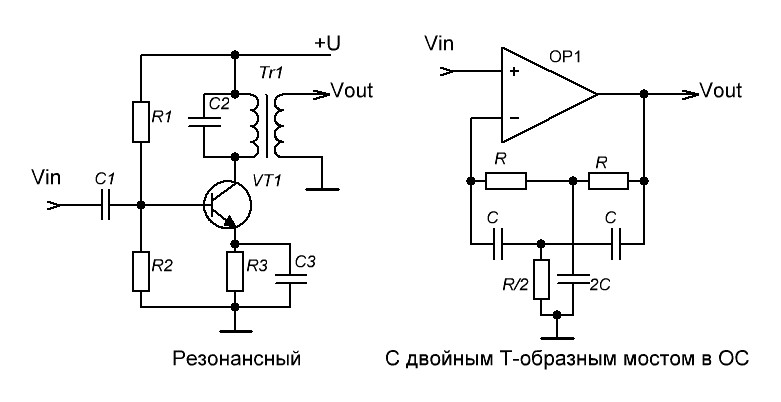
\includegraphics[width=0.6\textwidth]{146.jpg}
\caption{Избирательные усилители}
\end{figure}

% Вопрос 147 --------------------------------------------------------
\quest{Схема стабилизатора напряжения на 10 В, 2 А на ИС К142.}

% Вопрос 148 --------------------------------------------------------
\quest{Схема стабилизатора напряжения на 12 В, 1 А на ИС К142.}

% Вопрос 149 --------------------------------------------------------
\quest{Схема ключевого стабилизатора напряжения.}

% Вопрос 150 --------------------------------------------------------
\quest{Генератор гармонических колебаний на транзисторах.}


% Вопрос 151 ----------------------------------------------------------
\quest{Системы хранения данных. Назначение. Три основные структуры систем хранения данных.}

С ростом производительности ЭВМ и увеличением объемов хранимой информации возникает необходимость в специальных внешних устройствах для хранения данных. ВЗУ большого объема обычно строятся на основе ленточных накопителей, которые обладают большим временем доступа и быстрым старением. Возникает задача хранения больших объемов данных с быстрым временем доступа.

Причинами появления СХД считают следующие: децентрализация хранения информации (организациям со временем приходится задействовать оборудование филиалов для хранения информации), низкий уровень защиты данных, низкая степень конфиденциальности передаваемых данных, требования к масштабируемости (неизвестно какие объемы информации потребуется хранить через несколько лет). Возникает необходимость в некой автоматизированной системе, которая хранила бы данные.

В простейшем случае структуру такой системы можно представить в следующем виде: \mbox{SCSI --- RAID-контроллер --- HDD (несколько)}.

К SCSI подключается RAID-контроллер с буферным каналом ввода/вывода и кэш-памятью достаточно большого объема. Задача RAID- контроллера обеспечить формирование RAID- массива: присваивание файлам своих адресов. Связь контроллера с HDD осуществляется по параллельным линиям с электрическими или оптическими сигналами.

За счет кэш-памяти RAID-контроллер обеспечивает высокую скорость доступа к данным, при этом задача буферного блока скомпоновать общий файл при нескольких запросах. Кроме того, в буферном блоке производится контроль информации, при необходимости с восстановлением.

Такие СХД подключаются к типовым интерфейсам, прежде всего к SCSI (до 640 Мб/с). Помимо него часто используется Fibre Channel --- интерфейс с оптическими линиями связи способный обеспечивать до 4 Гб/с.

\textbf{Структура СХД}. Для подключения внешних дисков требуется внешний контроллер с высоким быстродействием, чтобы обеспечить приемлемую скорость передачи массива. Передача идет файлам не непрерывно, с попеременными чтением и записью, поэтому в структуру СХД должны входить следующие блоки:

\begin{figure}[H]
\centering
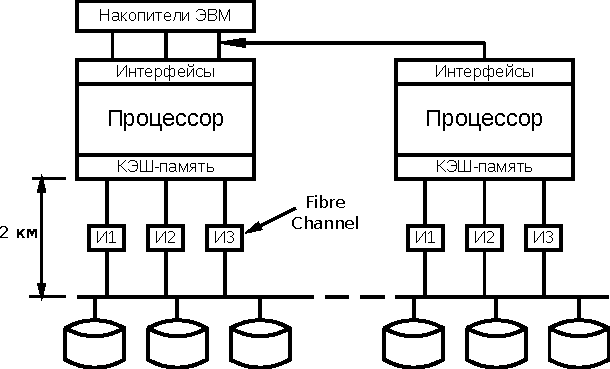
\includegraphics[width=0.6\textwidth]{151_struct.pdf}
\caption{Структура СХД}
\end{figure}

Процессор контроллера должен обладать высокой переключающей способностью, а интерфейс к ЭВМ должен позволять пересылать большие массивы данных. Связь со стойками с дисками невозможна без буферной памяти.

Информацию при передаче данных можно восстановить, но сбой при записи может привести к потере данных, поэтому система резервируется. Одновременно работают два контроллера, но доступ отдан одному. В случае возникновения ошибки, второй контроллер вступает в работу, его кэш-память так же страхует возможные потери информации.

Такие структуры входят в состав стоек, и часто не одна система хранения данных, а несколько, как бы отдельных.

\textbf{Организация СХД}. В зависимости от объемов хранимой информации, сложности системы и требований к надежности можно выделить три основные структуры СХД:

\textit{Прямое включение <<DAS>>}. Сервер сети и сервер СХД разделены. Имеется толь одна линия доступа к СХД, что снижает надежность в случае отказа и скорость доступа к данным.

\begin{figure}[H]
\centering
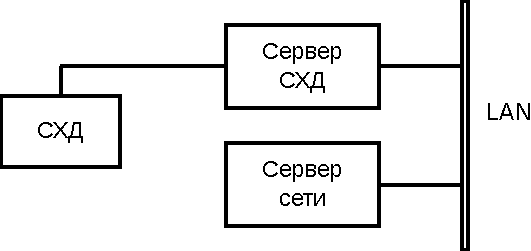
\includegraphics[width=0.4\textwidth]{151_das.pdf}
\caption{Прямое включение <<DAS>>}
\end{figure}

\textit{Прямое подключение в сеть <<NAS>>}. СХД является абонентом сети, обеспечивающим файловый доступ, и должна иметь соответствующее сетевое оборудование. У каждой стойки может быть свое особенное ПО.

\begin{figure}[H]
\centering
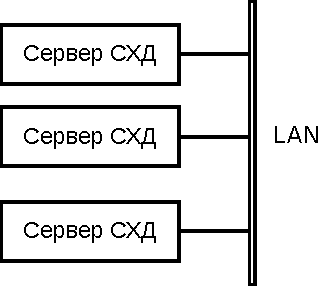
\includegraphics[width=0.25\textwidth]{151_nas.pdf}
\caption{Прямое подключение в сеть <<NAS>>}
\end{figure}

\textit{Сетевое подключение <<SAN>>}. Имеется возможность переключения каналов передачи информации. СХД подключается сразу к 2 каналам и, если один из них загружен, то используется второй. Система централизованная, но сложная и дорогая.

\begin{figure}[H]
\centering
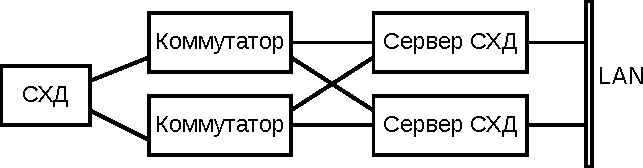
\includegraphics[width=0.6\textwidth]{151_san.pdf}
\caption{Сетевое подключение <<SAN>>}
\end{figure}


% Вопрос 152 ----------------------------------------------------------
\quest{Основные понятия информационно-вычислительных систем, классификация по критерию потоков информации.}

Понятие вычислительная машина обычно применяют к вычислительному устройству, имеющему небольшие габариты и единую конструкцию. Обычно это устройство включает минимально необходимые функциональные узлы. Система относится к более сложным устройствам и объединяет функциональные блоки территориально разнесенные, чаще однотипные. В составе системы может быть несколько функциональных однотипных блоков. Понятие комплекс выше системы, его применяют к устройствам занимающим определенное пространство, т.е. разнесенные, имеющие каналы связи и разнотипные повторяющиеся функциональные блоки. Поскольку между комплексом и системой граница размыта, обычно их разделяют по конструктивному признаку. \textbf{Комплекс} --- это множество самостоятельных конструктивно устройств. \textbf{Сети} --- территориально разнесенные вычислительные устройства, использующие стандартные способы связи между собой.

Как правило, информационно- вычислительная система (ИВС) или информационно- вычислительный комплекс (ИВК) имеют прикладное назначение. Те или иные конфигурации предназначены для сбора и обработки информации, управления, диагностирования, автоматизированных рабочих мест. В этих структурах непосредственно вычислительные процедуры занимают не основную роль. Основным становится передача, хранение информации. В зависимости от состава системы изменяется конфигурация, динамические характеристики, надежность устройств. В процессе эволюции системы прошли длинный путь, поэтому появились различные конфигурации вычислительных систем.

\textbf{Классификация по потокам информации (по Флину)}

В любой ВС можно выделить два основных информационных потока: поток команд и поток данных, поэтому представляется 4 основных конфигурации:

\begin{enumerate}
\item ОКОД. Один поток команд, один поток данных.

Один процессор с раздельными памятью команд и данных. Это последовательная структура, в которой данные связаны с одной конкретной командой. Если необходимы новые данные, формируется новая команда или повторяется.

\begin{figure}[H]
\centering

\includegraphics[width=0.45\textwidth]{152_okod.pdf}
\caption{Организация ВС: один поток команд, один поток данных}
\end{figure}

\item ОКМД. Один поток команд, множество потоков данных.

Специализированные микропроцессоры использующиеся для параллельной обработки различных данных по одной команде. Эта структура наиболее близка к термину параллельная обработка, поскольку в каждый момент времени множество операндов преобразуются под управлением одинаковых команд. Параллельные системы с такой структурой применяют для обработки многомерной графики, сигналов от реальных датчиков, работающих в реальном времени.

\begin{figure}[H]
\centering
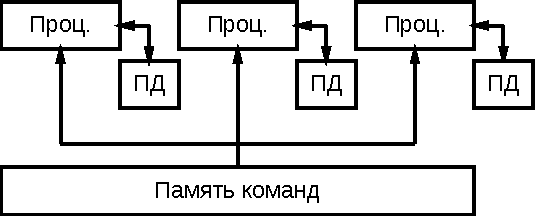
\includegraphics[width=0.45\textwidth]{152_okmd.pdf}
\caption{Организация ВС: один поток команд, множество потоков данных}
\end{figure}

\item МКОД. Множество потоков команд, один поток данных.

Конвейерная структура реализованная непосредственно на кристалле. Процессоры соединены в цепочку по шинам данных, при этом шины команд у каждого самостоятельные. В каждый момент времени выполняются разные команды в процессорах над одним потоком данных. Поток данных в этом случае --- последовательность операндов несущих информацию о какой-то величине. При этом каждое значение операнда последовательно преобразуется согласно поступающим командам.

\begin{figure}[H]
\centering
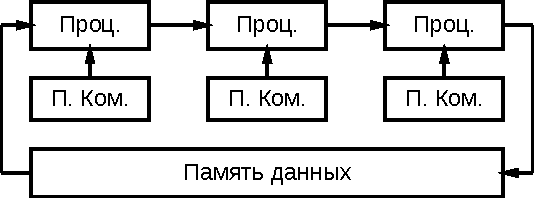
\includegraphics[width=0.45\textwidth]{152_mkod.pdf}
\caption{Организация ВС: множество потоков команд, один поток данных}
\end{figure}

\item МКМД. Множество потоков команд, множество потоков данных.

Матричная регулярная структура, где матрица процессоров в одном слое использует параллельную обработку, а последовательно по слоям --- конвейер. Такие структуры известны как однородные вычислительные системы. Применяются в сверхбыстродействующих специализированных системах работы с реальными сигналами.

\begin{figure}[H]
\centering
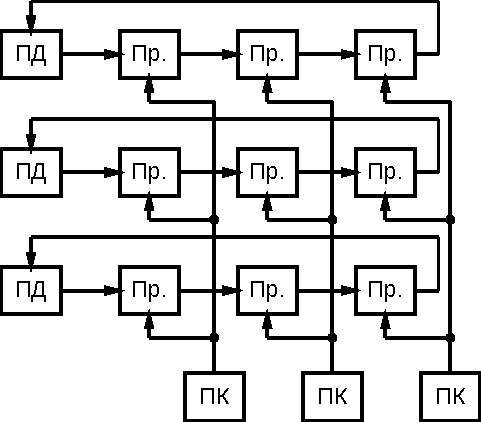
\includegraphics[width=0.45\textwidth]{152_mkmd.pdf}
\caption{Организация ВС: множество потоков команд, множество потоков данных}
\end{figure}

\end{enumerate}


% Вопрос 153 ----------------------------------------------------------
\quest{Совмещение операций и многопрограммная работа. Режим работы в реальном времени.}

Режим работы ЭВМ --- это порядок прохождения задач (заданий) через ЭВМ. Задача --- это программа и данные, загруженные в ОП, т.е. программа вместе с выделенными ей ресурсами. Различают режимы работы двух типов --- однозадачный (однопрограммный) и мультизадачный (мультипрограммный).

В \textit{однопрограммном режиме} аппаратура ЭВМ выполняет одну пользовательскую программу под управлением и с использованием программ ОС. Практически это двухпрограммный режим: пользовательская программа плюс программа ОС. Но поскольку программы ОС являются сервисными, обслуживающими запросы пользователя, такой режим называют однопрограммным (однозадачным).

\begin{figure}[H]
\centering
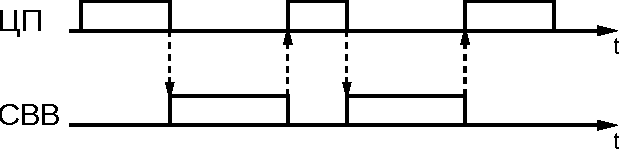
\includegraphics[width=0.5\textwidth]{153_single.pdf}
\caption{Диаграмма загруженности ЭВМ в однопрограммном режиме}
\end{figure}

Основное \textit{достоинство однопрограммного режима} --- минимальное время ответа на запросы пользователя. Все ресурсы ЭВМ (и аппаратные, и программные) находятся в распоряжении пользователя --- нет конкуренции за ресурсы. Пользователь монопольно владеет всеми ресурсами.

Основной \textit{недостаток однопрограммного режима} --- неэффективное использование оборудования, в частности, процессора: как видно из временной диаграммы, большую часть времени процессор простаивает.  Быстродействие системы ввода/вывода, обычно существенно ниже быстродействия процессора и памяти.

Как вариация однопрограммного режима существует \textit{пакетный режим}: в этом режиме пользователь подготавливает последовательность (пакет) запускаемых по очереди программ, что исключает ожидание ввода пользователя для запуска каждой последующей программы. Это несколько повышает реальную производительность системы.

В более мощных, дорогих ЭВМ с целью повышения эффективности использования оборудования применяется \textit{мультипрограммный режим}. В этом режиме, кроме программ ОС, в ОП компьютера располагаются и (по очереди) выполняются несколько (в общем случае М) программ пользователей, при этом, пока одна из программ ожидает завершения операций ввода/вывода, управление передаётся другой программе. Цель --- увеличение загрузки ЦП и, как следствие, производительности ЭВМ.

\begin{figure}[H]
\centering
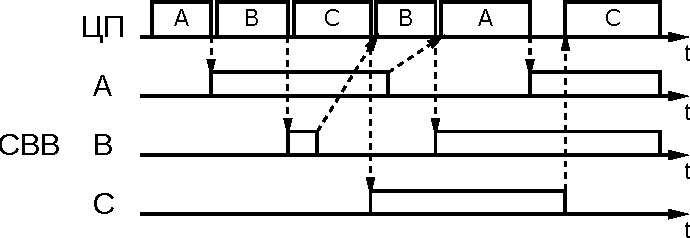
\includegraphics[width=0.6\textwidth]{153_multi.pdf}
\caption{Диаграмма загруженности ЭВМ в многопрограммном режиме}
\end{figure}

Мультипрограммный режим сложнее однопрограммного, поэтому к ВС предъявляет специальные требования. Для их реализации в состав ЭВМ вводятся специальные средства, которые и принято называть средствами мультипрограммирования. Средства, обеспечивающие заданный режим мультипрограммирования --- это управляющие программы ОС. Они обеспечивают требуемый порядок прохождения задач через ЭВМ, образуют основную часть --- ядро ОС.

\textit{Режим реального времени} применяют в вычислительных системах, работающих с физическими сигналами --- информационно-контролирующими, управляющими, обрабатывающими программами. Понятие это условно, поскольку время изменяется. Условие реального времени $ t_\text{обр.} < t_\text{пер.след.вх.сигн.}$. В этом режиме в первую очередь требуется быстрое измерение сигнала и занесение его в память, поэтому время начала работы процессора определяется временем поступления входного сигнала. Программа запускается по какому-то внешнему событию (чаще прерыванию).


\quest{Типы структур многопроцессорных ВС. Параллельные ЭВМ, классификация. Три архитектурных класса машин.}
\quest{Принципы ввода-вывода информации в ПЭВМ. Роль и структура контроллера ввода информации.}



% Вопрос 156 ----------------------------------------------------------
\quest{Программная реализация ввода чисел с клавиатуры. Привести алгоритм ввода двухразрядного числа с клавиатуры для его суммирования с другими числами.}

Принцип действия универсальной клавиатуры основан на формировании клавиатурного прерывания при нажатии клавиши. Клавиатурное прерывание является внешним и имеет свой вектор. Получив запрос на прерывание, процессор завершает текущую операцию, читает порт клавиатуры (60h) и переписывает код клавиши в буфер клавиатуры, расположенный в области данных BIOS в ОЗУ.
Чтение из буфера можно произвести с помощью стандартных подпрограмм BIOS (int 16h) и DOS (int 21h). В зависимости от подпрограммы процессор читает из буфера один символ (например: mov ah,00h; int 16h) или последовательность символов (например: mov ah,3fh; int 21h).

Т.к. использование таких функций позволяет получить коды символов, то для возможности работы с введенным числом необходимо преобразовать коды символов в двоичный код.  Алгоритм ввода двухразрядного числа для последующей работы с ним ([30h, 39h] — диапазон ASCII-кодов цифр):

Ожидать нажатия клавиши; Сохранить в регистре код нажатой клавиши; Проверить вхождение кода в диапазон [30h, 39h] (если не входит, вывести ошибку, повторить ввод); Отнять от кода 30h; Умножить код на 10; Переслать код в ячейку памяти; Ожидать нажатия клавиши; Сохранить в регистре код нажатой клавиши;  Проверить вхождение кода в диапазон [30h, 39h] (если не входит, вывести ошибку, повторить ввод); Отнять от кода 30h; Прибавить код к содержимому ячейки памяти;


\quest{Вывод информации на дисплей. Принципы отображения информации на экране дисплея. LCD- дисплеи.}
\quest{Процедура вывода символьной информации на дискретные индикаторы.}
\quest{Загрузчики. Процедура загрузки. Статические и динамические загрузки.}


% Вопрос 160 ----------------------------------------------------------
\quest{Управление реальной памятью. Виртуальная память. Таблица соответствия адресов.}

В многопрограммном режиме работы возникает задача размещения загружаемых программ в ОЗУ.  Участки памяти, куда загружаются программы, определяются с помощью программы управления памятью — диспетчера памяти. В зависимости от сложности задачи выделяют несколько стратегий управления памятью:

\textit{Статическое деление} --- разделение памяти на участки фиксированного объема, обычно применяется в простейших случаях (2-3 программы). Если процессов много, часть из них должна ожидать своей очереди для размещения в памяти, пока не завершатся предыдущие загруженные программы. Загрузка программы возможна только в том случае, если объем раздела в памяти больше объема программы, следовательно с такой системой загрузки всегда остается неиспользуемое свободное место в памяти, что снижает эффективность ее использования.

\textit{По запросу} --- деление памяти на фрагменты переменной длины. Процессы стоящие в очереди получают необходимый для загрузки объем памяти, следовательно память используется эффективнее. Когда один или несколько процессов завершатся, в освободившуюся область памяти загружаются новые процессы из очереди, которые однако имеют другой размер, поэтому в занимаемой памяти образуются <<дыры>>. Чтобы исправить эту проблему производится \textit{дефрагментация} --- сдвиг одного из массивов к окончанию другого. При этом возникает задача нахождения в кодах абсолютных ссылок и изменения их, для их нахождения команды переходов по абсолютным адресам могут быть отмечены специальным битом (технически это не предусмотрено в системе команд) либо при компиляции в конец файла могут быть записаны адреса таких команд. Для выполнения дефрагментации требуется специальная программа для пересылки массивов.

Другая проблема возникает, когда работающий процесс затребовал дополнительную память, поэтому массив новых данных формируется в другом сегменте памяти. В таком случае программа управления памятью работает как редактор связей: делает ссылку в текущих кодах на новое адресное пространство.

Загрузку программ в память выполняет загрузчик, который выполняет пересылку по необходимым адресам. Загрузка в память выполняется по параграфам (младшая тетрада адреса загрузки равна нулю). Загрузка может производиться в статическом (сначала загружаются все задачи, затем выполняются), либо в динамическом (в промежутках между работой загружаются другие задачи) режимах.

Основная память ВС ограничена, в то же время используя ВЗУ можно попеременно по одним и тем же адресам в основной памяти загружать коды из внешней памяти и работать с ними. Такую организацию памяти называют \textit{виртуальной}. Основная проблема при таком алгоритме работы — связывание конкретной задачи с адресами в ВЗУ. Кроме того, при работе с файлам может возникнуть необходимость сохранения их в ВЗУ, для этого используется таблица соответствия адресов.

\begin{figure}[H]
\centering
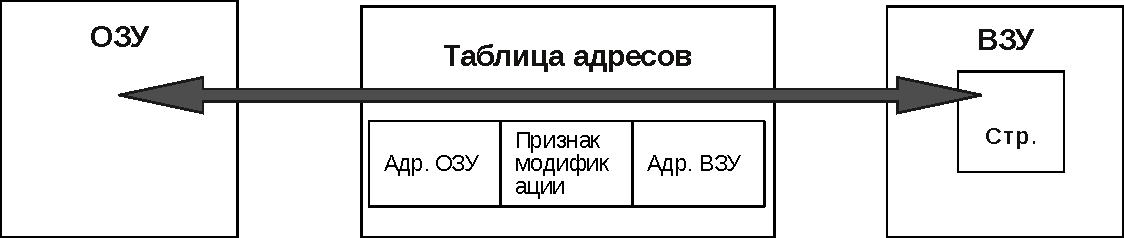
\includegraphics[width=0.7\textwidth]{160_virtual_memory.pdf}
\caption{Схема работы с виртуальной памятью}
\end{figure}

\end{document}
